% !TEX program = pdflatex
\documentclass[journal]{IEEEtran}

% ──────────────────────────────────────────────────────────────────────────────
%  Packages
% ──────────────────────────────────────────────────────────────────────────────
\usepackage[T1]{fontenc}
\usepackage{amsmath,amssymb,amsfonts}
\usepackage{algorithmic}
\usepackage[ruled,linesnumbered]{algorithm2e}
\usepackage{graphicx}
\usepackage{textcomp}
\usepackage{xcolor}
\usepackage{booktabs}
\usepackage{multirow}
\usepackage{hyperref}
\usepackage{cleveref}
\usepackage{bm}
\usepackage{mathtools}
\usepackage{subcaption}
\usepackage{siunitx}
\usepackage{balance}

% Theorem environments
\newtheorem{theorem}{Theorem}
\newtheorem{lemma}[theorem]{Lemma}
\newtheorem{corollary}[theorem]{Corollary}
\newtheorem{definition}[theorem]{Definition}
\newtheorem{remark}{Remark}
\newtheorem{assumption}{Assumption}

% Notation shortcuts
\newcommand{\Cfree}{\mathcal{C}_{\mathrm{free}}}
\newcommand{\Cspace}{\mathcal{C}}
\newcommand{\IR}{I_{\!R}}
\newcommand{\IE}{I_{\!E}}
\newcommand{\dR}{d_{\!R}}
\newcommand{\SPD}{\mathbb{S}_{++}^{d}}
\newcommand{\muR}{\mu_{\!R}}
\newcommand{\Vol}{\mathrm{Vol}}
\newcommand{\diag}{\mathrm{diag}}
\DeclareMathOperator*{\argmin}{arg\,min}

% IEEE specific
\IEEEoverridecommandlockouts

\begin{document}

% ══════════════════════════════════════════════════════════════════════════════
%  TITLE
% ══════════════════════════════════════════════════════════════════════════════
\title{RIT*: Riemannian Informed Trees for\\Sampling-Based Motion Planning}

\author{
  \IEEEauthorblockN{Author~Names~Omitted~for~Review}
  \IEEEauthorblockA{Affiliation Omitted for Review}
}

\markboth{IEEE Robotics and Automation Letters}{Author~et~al.: RIT*: Riemannian Informed Trees}

\maketitle

% ══════════════════════════════════════════════════════════════════════════════
%  ABSTRACT
% ══════════════════════════════════════════════════════════════════════════════
\begin{abstract}
Finding optimal collision-free paths in high-dimensional configuration
spaces is central to robot manipulation, yet remains computationally
challenging.
State-of-the-art asymptotically-optimal planners---Informed~RRT*,
BIT*, AIT*, EIT*, and the recent APT*---accelerate convergence by
focusing sampling within an informed set, but all define this set
using Euclidean distance. When traversal costs are anisotropic or
spatially varying (e.g.\ joint-inertia weighting, obstacle-proximity
penalties), the Euclidean informed set is a strict superset of the
true cost-relevant region, wasting samples and slowing convergence.
Moreover, no existing planner can learn a suitable cost metric online.
We present \textbf{RIT*} (Riemannian Informed Trees), a unified
planning framework that replaces every Euclidean primitive in the
batch-informed pipeline---informed set, neighbourhood ball, and edge
cost---with its Riemannian counterpart, and learns the cost landscape
online when no a~priori metric is available. A whitening transform
enables efficient uniform sampling from the tighter Riemannian
informed set; a cascading three-level edge evaluation (midpoint,
Simpson, Gauss--Legendre) filters ${\sim}95\%$ of candidate edges
before expensive integration; and an integrated Collision-Adaptive
Riemannian Metric (CARM) module constructs the metric online from
collision feedback via kernel density estimation, eliminating the need
for a~priori obstacle knowledge.
Experiments across 14~environments (2-D through 6-DOF UR10e
manipulator) with five Monte Carlo trials per configuration against
five baselines show that RIT*-CARM achieves the lowest cost on 11 of
14~environments---up to 70\% cost reduction in 6-D---while RIT* with
a pre-defined joint-inertia metric achieves up to 15\% improvement
on 6-D manipulator tasks without online learning.
\end{abstract}

\begin{IEEEkeywords}
Motion planning, Riemannian geometry, asymptotic optimality,
informed sampling, online metric learning, manipulator planning.
\end{IEEEkeywords}

\begin{figure*}[t]
\centering
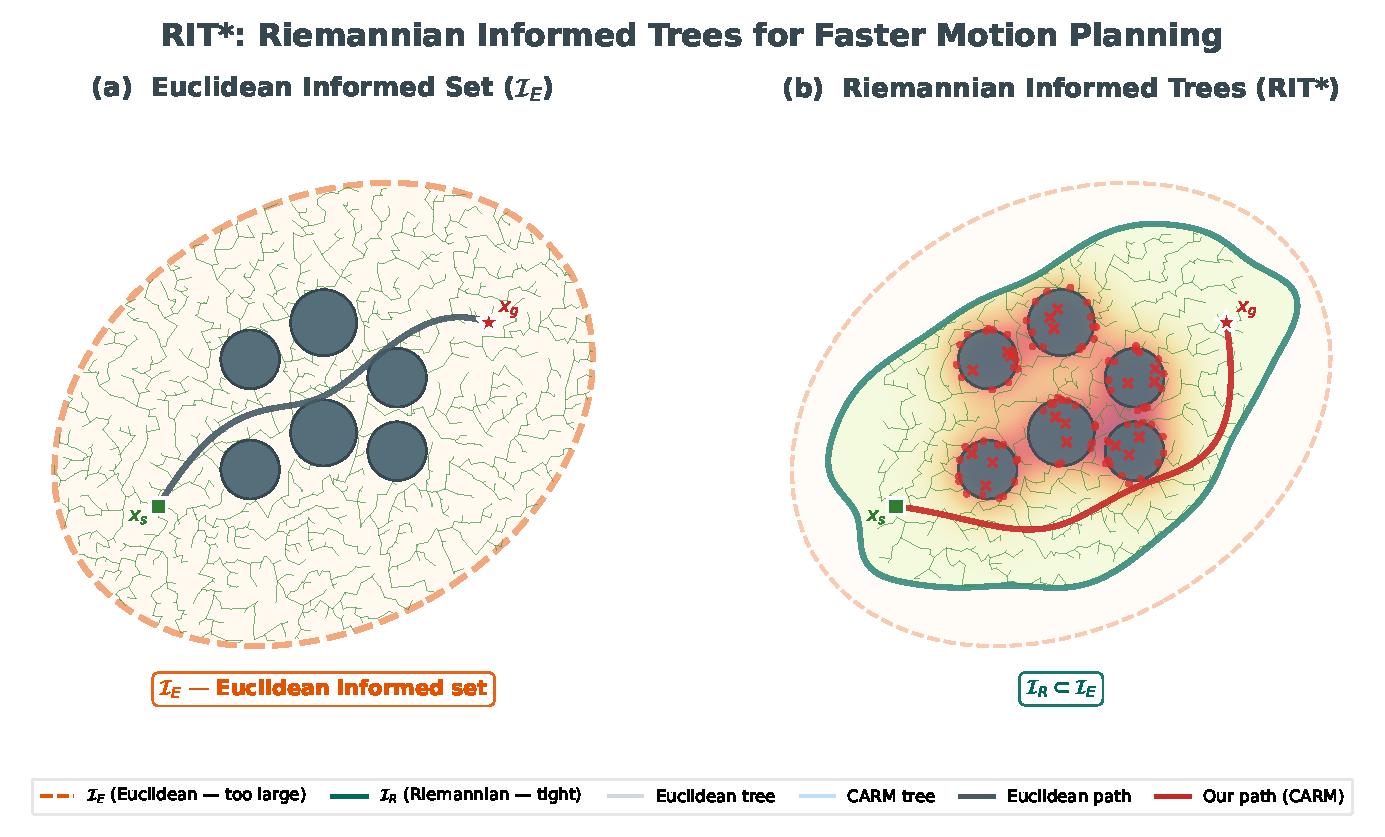
\includegraphics[width=\textwidth]{figures/fig_abstract.pdf}
\caption{Overview of RIT* on a 2-D obstacle environment.
  \textbf{(a)}~Standard Euclidean planners sample uniformly from the
  large informed set~$\mathcal{I}_E$ (orange dashed ellipse), wasting
  many samples in high-cost regions near obstacles. The isotropic
  neighborhood ball~$r_n$ (circle) treats all directions equally.
  \textbf{(b)}~RIT* replaces every Euclidean primitive with its
  Riemannian counterpart: the tighter informed set~$\mathcal{I}_R
  \subset \mathcal{I}_E$ (teal) eliminates up to 71\% of wasted
  volume; the anisotropic neighborhood ball~$r_n^R$ (ellipse) reaches
  further along cheap directions; a three-level cascading filter
  rejects ${\sim}95\%$ of candidate edges before expensive integration;
  and the integrated CARM module learns a cost field online from
  collision feedback ($s(x) = 1 + \alpha\hat{f}(x)$, warm-color
  heatmap), progressively tightening $\mathcal{I}_R$ and steering
  samples away from obstacles without any a~priori obstacle model.}
\label{fig:abstract}
\end{figure*}

% ══════════════════════════════════════════════════════════════════════════════
%  I. INTRODUCTION
% ══════════════════════════════════════════════════════════════════════════════
\section{Introduction}\label{sec:intro}

Sampling-based motion planning is a cornerstone of robotics, enabling
collision-free path computation in high-dimensional configuration
spaces~\cite{LaValle2006}. The introduction of asymptotically-optimal
(AO) planners---RRT*~\cite{Karaman2011} and PRM*---established that
random sampling can converge almost surely to the optimal
path. Subsequent work accelerated convergence through \emph{informed
sampling}: once an initial solution of cost $c_{\mathrm{best}}$ is
found, new samples are drawn only from the \emph{informed set}
$\IE = \{ x : \|x_s - x\|_2 + \|x - x_g\|_2 \le c_{\mathrm{best}} \}$,
a prolate hyperspheroid in Euclidean space~\cite{Gammell2018}.
This idea underpins Informed~RRT*~\cite{Gammell2018},
BIT*~\cite{Gammell2020}, AIT* and EIT*~\cite{Strub2022}, and the
recent APT*~\cite{APT2025}.

All of these planners assume the cost is Euclidean: traversal cost
equals arc length. In practice, costs are often
\emph{anisotropic}---joint-inertia weighting, obstacle-proximity
penalties~\cite{Ratliff2009,Zucker2013}, task-space norms---making them
naturally Riemannian. When the cost is Riemannian, the Euclidean informed
set $\IE$ is a \emph{strict superset} of the true informed set: it wastes
samples in regions where the Riemannian cost is too high for path
improvement.

\textbf{Contributions.}
We propose \textbf{RIT*}, a unified Riemannian planning framework
that replaces $\IE$ with the \emph{Riemannian informed set}
\begin{equation}\label{eq:IR}
  \IR = \bigl\{ x \in \Cspace : \dR(x_s, x) + \dR(x, x_g) \le c_{\mathrm{best}} \bigr\},
\end{equation}
and integrates Riemannian geometry into every stage of the
batch-informed planning pipeline---including online metric learning
when no a~priori metric is available. Our specific contributions are:

\begin{enumerate}
  \item \textbf{Riemannian informed planning pipeline.}
    We replace every Euclidean primitive in the batch-informed pipeline
    with its Riemannian counterpart: (i)~a whitening transform
    $\tilde{x} = G^{1/2}\,x$ maps $\IR$ to a standard prolate
    hyperspheroid for efficient uniform sampling;
    (ii)~neighbours are found within ellipsoidal Riemannian balls
    whose axes align with the metric eigenvectors, naturally reaching
    further along cheap directions; and (iii)~a three-level cascading
    edge evaluation scheme---midpoint (L1), Simpson's rule (L2),
    Gauss--Legendre quadrature (L3)---filters ${\sim}95\%$ of
    candidate edges before expensive integration. This is the first
    integration of Riemannian geometry into the \emph{global}
    informed sampling strategy of a batch-informed planner.

  \item \textbf{Online metric learning via CARM.}
    As an integral part of RIT*, the Collision-Adaptive Riemannian
    Metric (CARM) module constructs a Riemannian cost field online
    from collision feedback using kernel density estimation,
    eliminating the need for a~priori obstacle knowledge. Unlike
    prior obstacle-aware Riemannian
    metrics~\cite{Klein2023,BeikMohammadi2023} that require known
    obstacle geometry or demonstrations, CARM learns purely from the
    binary collision checker already available to any sampling-based
    planner, and feeds the learned metric directly into the informed
    set, neighbourhood, and pruning operations.

  \item \textbf{Comprehensive experimental evaluation.}
    We evaluate RIT* across 14~environments (6$\times$2-D,
    4$\times$3-D, 4$\times$6-D including UR10e manipulator) against
    five baselines spanning 2011--2025, with five Monte Carlo trials
    per configuration. RIT*-CARM achieves the lowest cost on 11 of
    14~environments, with up to 70\% cost reduction in 6-D. On
    manipulator tasks with a known joint-inertia metric, RIT* achieves
    up to 15\% improvement without any online learning.
\end{enumerate}

\begin{figure*}[t]
\centering
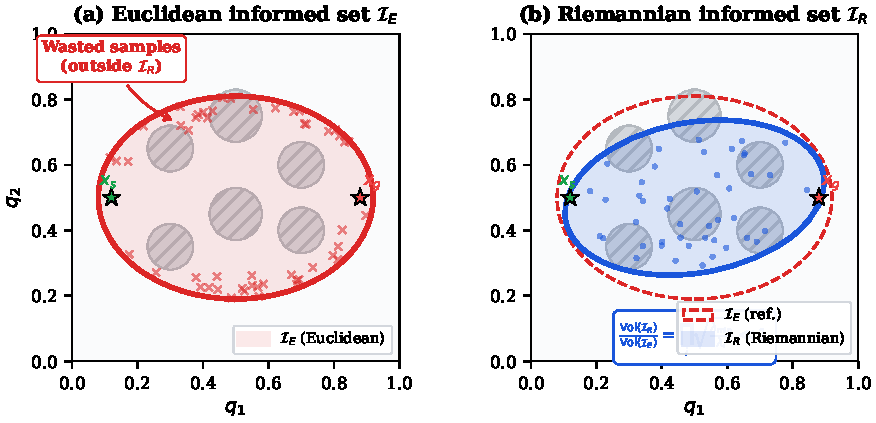
\includegraphics[width=\textwidth]{figures/fig_informed_sets.pdf}
\caption{Comparison of Euclidean and Riemannian informed sets.
  (a)~The Euclidean informed set $I_E$ (red ellipse) wastes samples in
  regions where the Riemannian cost is too high for path improvement.
  (b)~The Riemannian informed set $I_R$ (blue ellipse) is shaped by
  the metric tensor, focusing samples on the subspace that can
  actually contain improving paths.}
\label{fig:informed_sets}
\end{figure*}

\subsection{Related Work}\label{sec:related}

\textbf{Euclidean informed sampling planners.}
Gammell~et~al.~\cite{Gammell2018} introduced direct sampling of the
prolate hyperspheroid, accelerating RRT* convergence.
BIT*~\cite{Gammell2020} combines batch sampling with informed sets and
lazy edge evaluation.  AIT* and EIT*~\cite{Strub2022} add asymmetric
bidirectional search with adaptive or effort-based heuristics.
APT*~\cite{APT2025} uses Coulomb-force-inspired virtual forces from
valid and invalid neighbour vertices to prolate the nearest-neighbour
ball into a direction-dependent ellipsoid, and adapts batch size via
the shrinking hypervolume of the Euclidean informed set.
FIT*~\cite{FIT2024} adjusts batch size for faster initial convergence.
All of these define the informed set, neighbourhood ball, and edge cost
in \emph{Euclidean} distance.

\textbf{Riemannian geometry in motion planning.}
CHOMP~\cite{Ratliff2009} and STOMP~\cite{Zucker2013} optimise
trajectories under Riemannian-like costs but are trajectory optimisers,
not sampling-based planners, and lack AO guarantees.
Jaillet and Sim\'{e}on~\cite{Jaillet2008} proposed cost-space RRT
variants. Kim~et~al.~\cite{Kim2016} used Riemannian metrics for local
steering on constrained manifolds but not for informed set construction.
Kyaw and Kelly~\cite{Kyaw2026} recently proposed a Riemannian RRT*
that uses Riemannian distance for local steering via retractions and
natural gradients; however, their planner is RRT*-based (not
batch-informed), does not construct an informed set, and does not employ
caching or cascading edge evaluation. Their future work explicitly
identifies ``heuristic functions in curved spaces to focus search'' as
an open problem---precisely the problem that RIT*'s Riemannian informed
set addresses.
Bi-AM-RRT*~\cite{Zhang2023biamrrt} uses a diffusion-based
``assisting metric'' to bias nearest-neighbour selection in RRT*, but
operates in an incremental (non-batch) framework without informed sets
or progressive edge evaluation.

\textbf{Obstacle-aware Riemannian metrics.}
Klein~et~al.~\cite{Klein2023} design region-avoiding Riemannian metrics
using hand-crafted barrier functions that guarantee strict obstacle
avoidance for geodesic-based trajectory generation on a humanoid robot.
Their approach requires full obstacle geometry a~priori, uses analytic
barrier functions (not learned kernels), and applies to trajectory
optimisation rather than sampling-based planning.
RMPflow~\cite{Cheng2018rmpflow} constructs Riemannian motion policies
for reactive control by composing task-space metrics; it is a local
reactive controller, not a global planner.
Beik-Mohammadi~et~al.~\cite{BeikMohammadi2023} learn Riemannian
manifolds from human demonstrations using a variational autoencoder
and reshape the learned manifold with an obstacle-aware ambient metric
for reactive motion generation. Their approach is demonstration-driven,
operates in a learned latent space, and does not integrate with
sampling-based planning.
RIT*'s integrated CARM module differs from all of these: it learns a
Riemannian metric \emph{online} from collision feedback (no a~priori
obstacle model, no demonstrations), uses kernel density estimation on
collision points, and feeds the learned metric directly into the
informed set, neighbourhood, and pruning operations of the
batch-informed planning loop.

\textbf{Key distinction.}
Prior Riemannian planning work uses the metric for \emph{local}
steering, trajectory optimisation, or reactive control. RIT* is the
first to integrate Riemannian geometry into the \emph{global} informed
sampling strategy---replacing the informed set, neighbourhood ball,
edge integration, and rewiring cost of a batch-informed planner with
their Riemannian counterparts---and to learn the metric online from
collision feedback via its integrated CARM module.


% ══════════════════════════════════════════════════════════════════════════════
%  II. PROBLEM FORMULATION
% ══════════════════════════════════════════════════════════════════════════════
\section{Problem Formulation}\label{sec:problem}

\subsection{Riemannian Configuration Space}

\begin{figure*}[t]
\centering
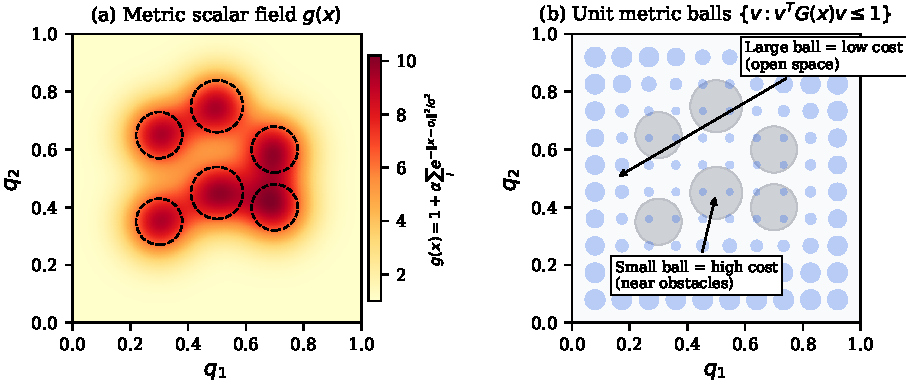
\includegraphics[width=\textwidth]{figures/fig_metric_field.pdf}
\caption{Metric tensor field for the 2-D Obstacles environment.
  (a)~The scalar field $g(x)$ inflates traversal cost near obstacles.
  (b)~Unit metric balls $\{v : v^\top G(x)\, v \le 1\}$: smaller balls
  near obstacles indicate higher traversal cost; larger balls in open
  space indicate cheaper movement.}
\label{fig:metric_field}
\end{figure*}

Let $\Cspace \subseteq \mathbb{R}^d$ be a $d$-dimensional configuration
space equipped with a smooth, positive-definite metric tensor field
$G : \Cspace \to \SPD$, where $\SPD$ denotes the cone of
$d \times d$ symmetric positive-definite matrices. The Riemannian
arc-length cost of a path $\sigma : [0,1] \to \Cspace$ is
\begin{equation}\label{eq:cost}
  c(\sigma) = \int_0^1 \sqrt{\dot{\sigma}(t)^\top G\bigl(\sigma(t)\bigr)\, \dot{\sigma}(t)}\; dt.
\end{equation}
The \emph{geodesic distance} between two configurations is
$\dR(x,y) = \inf_\sigma c(\sigma)$ over all paths
$\sigma : x \to y$. When $G(x) = I_d$ (the identity), $\dR$
reduces to Euclidean distance $\|x - y\|_2$.

\textbf{Examples.}
(i)~\emph{Diagonal anisotropy}: $G = \diag(\lambda_1, \ldots, \lambda_d)$
models joint-inertia weighting.
(ii)~\emph{Obstacle-inflated}: $G(x) = g(x) I_d$, $g(x) \ge 1$
penalises proximity to obstacles (conformal metric).
(iii)~\emph{Joint-inertia metric}: $G(q) = M(q)$ where $M$ is the
manipulator mass matrix, encoding dynamic effort.

\subsection{Optimal Motion Planning Problem}

Given start $x_s$ and goal $x_g$ in the obstacle-free space
$\Cfree \subseteq \Cspace$, find the path
\begin{equation}
  \sigma^* = \argmin_{\sigma \,:\, x_s \to x_g,\; \sigma \subset \Cfree} c(\sigma).
\end{equation}
A planner is \emph{asymptotically optimal} (AO) if its solution cost
$c_n \to c^* \coloneqq c(\sigma^*)$ almost surely as $n \to \infty$.

\subsection{Informed Sets}

After finding a feasible path of cost $c_{\mathrm{best}}$, only
configurations that could lie on a shorter path need be considered. The
\emph{Euclidean informed set} is
\begin{equation}\label{eq:IE}
  \IE = \bigl\{ x \in \Cspace : \|x_s - x\|_2 + \|x - x_g\|_2 \le c_{\mathrm{best}} \bigr\},
\end{equation}
a prolate hyperspheroid. The \emph{Riemannian informed set} is defined
analogously using geodesic distance~\eqref{eq:IR}. Since
$G \succeq \lambda_{\min} I_d$ implies $\dR(x,y) \ge \sqrt{\lambda_{\min}}\,\|x-y\|_2$,
we have the containment $\IR \subseteq \IE$ for any metric with
$\lambda_{\min} \ge 1$.

\textbf{Volume reduction.}
For constant metric $G \in \SPD$ with eigenvalues
$\lambda_1 \le \cdots \le \lambda_d$, the ratio
\begin{equation}\label{eq:vol_ratio}
  \frac{\Vol(\IR)}{\Vol(\IE)}
  = \prod_{i=1}^{d} \sqrt{\frac{\lambda_{\min}}{\lambda_i}}
\end{equation}
follows directly from the whitened coordinate transform
$\tilde{x} = G^{1/2} x$ (see \cref{sec:whitening}).
For a 6-DOF manipulator with joint-inertia condition number
$\kappa = 12$, the Riemannian set has approximately $0.29$ times
the volume of the Euclidean set, eliminating 71\% of wasted samples.

% ══════════════════════════════════════════════════════════════════════════════
%  III. ALGORITHM
% ══════════════════════════════════════════════════════════════════════════════
\section{Algorithm}\label{sec:algorithm}

\subsection{RIT* Overview}

\begin{figure*}[t]
\centering
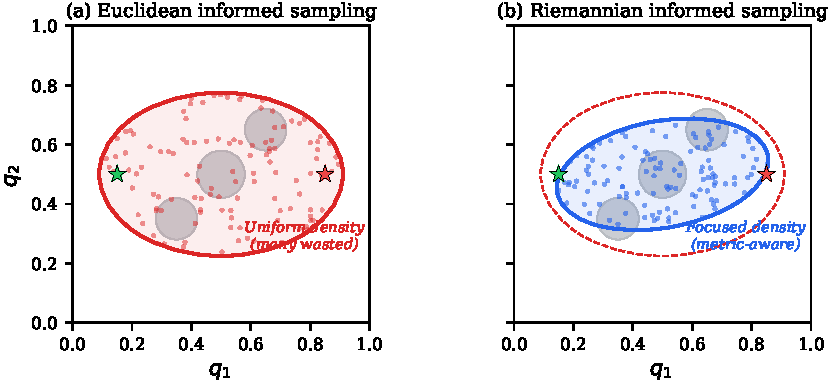
\includegraphics[width=\textwidth]{figures/fig_sampling.pdf}
\caption{Sampling strategies compared.
  (a)~Euclidean informed sampling draws uniformly from the prolate
  hyperspheroid $I_E$, wasting many samples in high-cost regions.
  (b)~Riemannian informed sampling draws from the tighter $I_R$,
  concentrating samples where they can improve the path.}
\label{fig:sampling}
\end{figure*}

\begin{figure*}[t]
\centering
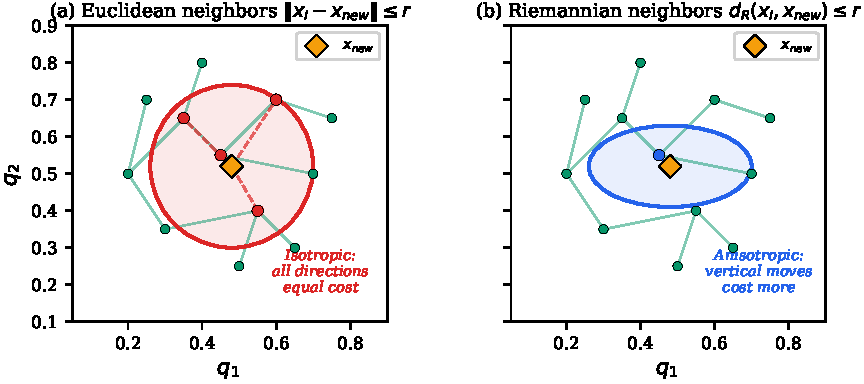
\includegraphics[width=\textwidth]{figures/fig_nearest_neighbor.pdf}
\caption{Nearest-neighbor selection.
  (a)~Euclidean neighbors within radius $r$: the isotropic ball treats
  all directions equally.
  (b)~Riemannian neighbors within $d_R \le r$: the anisotropic ball
  reaches further along cheap directions and less along costly ones,
  naturally adapting connectivity to the cost landscape.}
\label{fig:nearest_neighbor}
\end{figure*}

\cref{fig:pipeline} illustrates one iteration of RIT*.
\begin{figure*}[t]
\centering
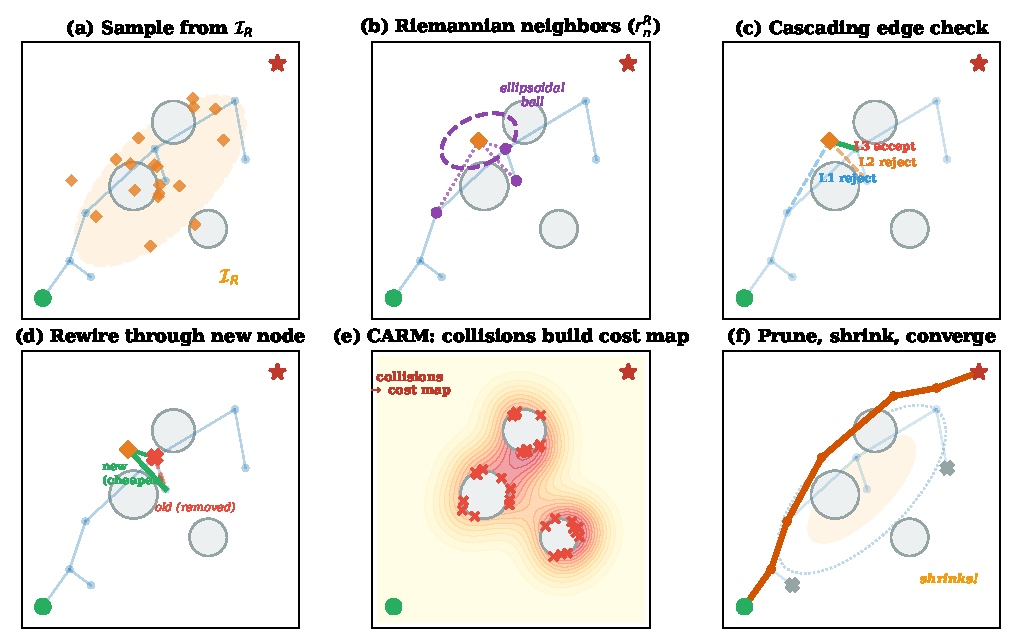
\includegraphics[width=\textwidth]{figures/fig_compact_pipeline.pdf}
\caption{Per-iteration pipeline of RIT*.
  (a)~A batch of samples is drawn from the Riemannian informed set
  $\mathcal{I}_R$, which concentrates samples where improvements are
  possible.
  (b)~Neighbors are found within ellipsoidal Riemannian radius $r_n^R$
  --- the ellipse stretches along inexpensive directions.
  (c)~Candidate parent edges are checked via a 3-level cascade: L1
  (midpoint) rejects most, L2 (Simpson) filters further, and only L3
  (Gauss--Legendre) uses full integration.
  (d)~The new node can provide cheaper paths to existing nodes;
  their parent edges are rewired (old edge removed, new edge
  established).
  (e)~Collision points from failed edge checks (red crosses) are fed
  to CARM, which builds a density-based cost field
  $s(x) = 1 + \alpha\hat{f}(x)$ that inflates traversal cost near
  obstacles.
  (f)~The informed set shrinks as $c_{\mathrm{best}}$ improves; nodes
  that cannot contribute to better paths are pruned.}
\label{fig:pipeline}
\label{fig:compact_pipeline}
\end{figure*}

\cref{fig:compact_pipeline} shows the six sub-steps of a single RIT*
iteration in detail, including the CARM feedback loop. We now describe
each step and the key modifications over BIT*.

\subsubsection{Step-by-step iteration}

\textbf{Sample (a).}
Before any solution is found ($c_{\mathrm{best}} = \infty$), samples
are drawn uniformly from $\Cspace$. Once a path is found, sampling
switches to the Riemannian informed set
$\IR = \{x : \dR(x_s, x) + \dR(x, x_g) \le c_{\mathrm{best}}\}$,
which is provably smaller than $\IE$~\eqref{eq:vol_ratio}.
For anisotropic metrics, the whitening transform makes
sampling from this non-standard shape efficient
(\cref{sec:whitening}).

\textbf{Find neighbors (b).}
For each new sample, we identify candidate parent nodes within
Riemannian distance $r_n^R$. Unlike the Euclidean ball (a sphere),
the Riemannian ball is an \emph{ellipsoid} whose axes align with
the metric eigenvectors: it reaches further along cheap directions
and less along expensive directions. This ensures that the most
relevant connections are considered first.

\textbf{Extend tree (c).}
Candidate parent edges are evaluated using a 3-level cascade.
Level~1 uses a single midpoint metric evaluation to reject
$\sim$80\% of candidates. Level~2 uses 3-point Simpson's rule to
filter a further $\sim$75\%. Only the surviving $\sim$5\% reach
Level~3 (10-point Gauss--Legendre quadrature) for exact cost
integration and collision checking.

\textbf{Rewire (d).}
After the new node is added, we check whether it offers cheaper
paths to nearby existing nodes. If
$g(x_{\mathrm{new}}) + c_R(x_{\mathrm{new}}, v) < g(v)$
for some neighbor $v$, then $v$'s parent is switched to
$x_{\mathrm{new}}$ and cost updates propagate to all descendants
of $v$ (\cref{fig:rewiring}).

\textbf{CARM feedback (e).}
During collision checks in steps (c) and (d), every collision point
is recorded and fed to CARM. Periodically (every $\Delta = 15$
iterations), CARM rebuilds its metric by placing Gaussian kernels on
each collision point to obtain a density
$\hat{f}(x) = N^{-1}\sum_i K_\sigma(x, c_i)$, then sets
$s(x) = 1 + \alpha \hat{f}(x)$. This inflates cost near obstacles,
tightening $\IR$ and steering future sampling away from cluttered
regions.

\textbf{Prune and update (f).}
After updating $c_{\mathrm{best}}$, nodes with
$f(v) = g(v) + h(v) > 1.05\, c_{\mathrm{best}}$ are
pruned. The informed set shrinks, and the next iteration samples from
the tighter region.

\begin{figure*}[t]
\centering
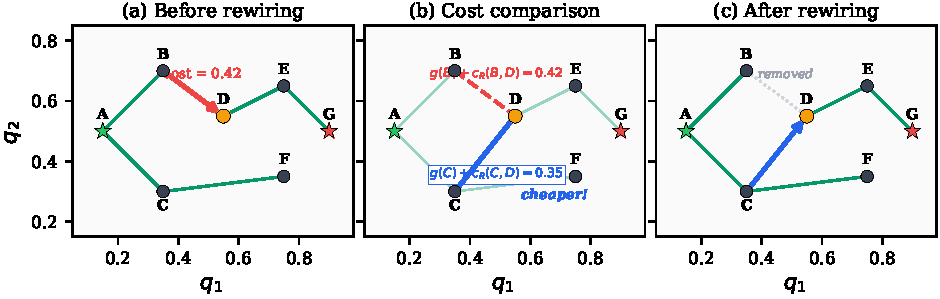
\includegraphics[width=\textwidth]{figures/fig_rewiring.pdf}
\caption{Tree rewiring step.
  (a)~Before rewiring: node~$D$ is connected to parent~$B$ with
  Riemannian edge cost 0.42.
  (b)~Cost comparison: the alternative parent~$C$ offers a cheaper
  connection ($g(C) + c_R(C,D) = 0.35$).
  (c)~After rewiring: $D$ is reconnected to~$C$, reducing the
  cost-to-come for all descendants.}
\label{fig:rewiring}
\end{figure*}

\subsection{Riemannian Informed Sampling via Whitening}\label{sec:whitening}

To sample uniformly from $\IR$, we transform to the whitened
coordinate system $\tilde{x} = G^{1/2} x$ where $\IR$ becomes a
standard prolate hyperspheroid. Uniform samples in whitened space are
mapped back via $G^{-1/2}$, yielding uniform coverage of $\IR$ in the
Riemannian volume measure (\cref{fig:whitening}).

\begin{figure*}[t]
\centering
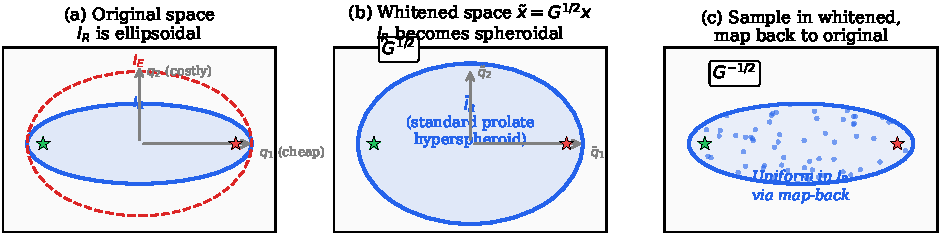
\includegraphics[width=\textwidth]{figures/fig_whitening.pdf}
\caption{Whitened coordinate sampling.
  (a)~In the original space, $I_R$ is a non-axis-aligned ellipsoid
  (hard to sample from directly).
  (b)~The whitening transform $\tilde{x} = G^{1/2} x$ maps $I_R$ to
  a standard prolate hyperspheroid.
  (c)~Uniform samples in whitened space are mapped back via $G^{-1/2}$,
  yielding uniform coverage of $I_R$ in the Riemannian volume measure.}
\label{fig:whitening}
\end{figure*}

\subsection{Cascading Lazy Edge Evaluation}

\begin{figure}[t]
\centering
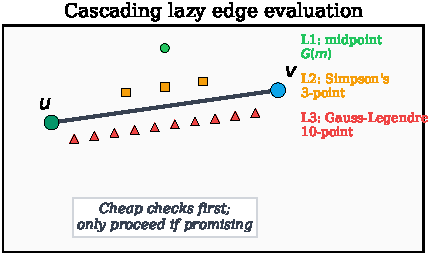
\includegraphics[width=\columnwidth]{figures/fig_edge_evaluation.pdf}
\caption{Cascading lazy edge evaluation. Edge cost is estimated at
  three levels of increasing accuracy: L1 (midpoint), L2 (Simpson's
  3-point), L3 (Gauss--Legendre 10-point). Cheap checks prune
  unpromising edges before expensive evaluations.}
\label{fig:edge_eval}
\end{figure}

Edge costs are evaluated in three levels of increasing accuracy:
(L1)~midpoint metric evaluation,
(L2)~3-point Simpson's rule, and
(L3)~10-point Gauss--Legendre quadrature. Cheap evaluations prune
unpromising edges before expensive evaluations are triggered.
The rationale is that Riemannian edge cost integration
$c_R(u,v) = \int_0^1 \sqrt{\dot\gamma^\top G(\gamma)\,\dot\gamma}\;dt$
is expensive---the cascading scheme amortises this cost by rejecting
most edges after a single metric lookup, reducing the average number of
$G(\cdot)$ evaluations per edge from 10 to approximately 1.6.

\subsection{Metric Tensor Field Cache}

A regular grid of resolution $\mathrm{res}^d$ stores precomputed
$G(x)$ values. Interpolation provides $O(1)$ lookups during planning,
avoiding repeated metric evaluations. Memory cost is
$O(\mathrm{res}^d \cdot d^2)$, negligible for $d \le 6$ at
$\mathrm{res} = 32$.

\subsection{Connection Radius}

The Riemannian connection radius is
\begin{equation}\label{eq:radius}
  r_n^R = \gamma_R \left(\frac{\log n}{n}\right)^{\!1/d}\!,\quad
  \gamma_R = 2\left(\frac{1}{d}\right)^{\!1/d}
             \!\left(\frac{\muR(\IR)}{\zeta_d}\right)^{\!1/d}
\end{equation}
where $\muR(\IR)$ is the Riemannian volume of the informed set and
$\zeta_d$ is the volume of the unit $d$-ball. Since
$\muR(\IR) < \mu(\IE)$, the Riemannian radius is smaller, yielding
fewer edges per vertex and faster per-iteration computation
(\cref{fig:connection_radius}).

\begin{figure}[t]
\centering
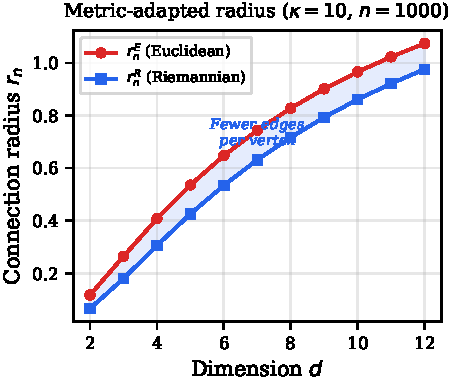
\includegraphics[width=0.7\columnwidth]{figures/fig_connection_radius.pdf}
\caption{Connection radius comparison for $\kappa=10$, $n=1000$.
  The Riemannian radius (blue) is smaller than the Euclidean radius
  (red) because $\muR(I_R) < \mu(I_E)$, yielding fewer edges per
  vertex and faster per-iteration computation.}
\label{fig:connection_radius}
\end{figure}

\begin{algorithm}[t]
\SetAlgoLined
\KwIn{$x_s, x_g, \Cfree, G(\cdot), B, T$}
\KwOut{optimal path $\sigma^*$}
$\mathcal{V} \gets \{x_s\}$; $\mathcal{E} \gets \emptyset$;
$c_{\mathrm{best}} \gets \infty$\;
Precompute metric cache $G[\cdot]$\;
\For{$t = 1, \ldots, T$}{
  $X_{\mathrm{new}} \gets \textsc{SampleRiemannianInformed}(B, c_{\mathrm{best}}, G)$\;
  $\mathcal{V} \gets \mathcal{V} \cup X_{\mathrm{new}}$\;
  \textsc{PruneNodes}$(\mathcal{V}, c_{\mathrm{best}}, G)$\;
  Compute $r_n^R$ via~\eqref{eq:radius}\;
  \ForEach{$v \in \mathcal{V}$ \textbf{in order of} $f(v)$}{
    $N(v) \gets$ neighbours within $r_n^R$ (Riemannian)\;
    \ForEach{$u \in N(v)$}{
      \If{\textsc{CascadingEdgeCheck}$(u, v, G)$}{
        Update tree $\mathcal{E}$;
        rewire neighbours\;
      }
    }
  }
  \If{$x_g$ reached with cost $c < c_{\mathrm{best}}$}{
    $c_{\mathrm{best}} \gets c$\;
    $\sigma^* \gets$ extract path\;
  }
  \textsc{CheckConvergence}$(t, c_{\mathrm{best}})$\;
}
$\sigma^* \gets \textsc{MultiStrategySmooth}(\sigma^*, G)$\;
\Return{$\sigma^*$}
\caption{RIT* planner}
\label{alg:ritstar}
\end{algorithm}

The per-iteration complexity is $O(n \log n)$, identical to BIT*.
The total number of samples for a given optimality gap is
$\kappa^{d/2}$ times smaller than Euclidean-informed planners, by
the volume reduction property~\eqref{eq:vol_ratio}.

\subsection{High-Dimensional Performance Engineering}\label{sec:highd}

Four targeted modifications address root causes of poor
high-dimensional performance in informed sampling planners:

\textbf{(H1) Dimension-adaptive stall threshold.}
The stall counter (iterations without improvement) triggers batch
resizing. In high-$d$, each batch explores a smaller fraction of the
exponentially larger space, causing premature stall detection.
We set $\tau_{\mathrm{stall}} = 5 + d$, allowing 11 stalls in 6-D
versus 5 in 2-D.

\textbf{(H2) Relaxed early stopping.}
Early stopping is disabled until $\max(30, T/3)$ iterations have
elapsed, preventing premature termination in high-$d$ where convergence
is inherently slower.

\textbf{(H3) Dimension-adaptive connection radius boost.}
The connection radius is scaled by
$\beta(d) = \max\bigl(1,\; 1 + 0.15(d-3)\bigr)$ for $d > 3$,
yielding a $1.45\times$ boost in 6-D. This counteracts the curse of
dimensionality: the probability of two random points being within
radius~$r$ decays as $r^d$, requiring larger radii to maintain tree
connectivity.

\textbf{(H4) Multi-strategy path smoothing.}
Post-processing applies three complementary strategies:
(i)~greedy forward shortcutting (skip maximal waypoints),
(ii)~greedy backward shortcutting (same, reversed direction), and
(iii)~random shortcutting with $\max(300, 100 d)$ attempts. This
replaces the single-strategy random shortcutting that is ineffective
in high dimensions.

\subsection{Metric Types Supported}

RIT* supports three classes of metric tensor fields:
(i)~\emph{constant diagonal} (joint inertia): exact volume
reduction~\eqref{eq:vol_ratio} applies;
(ii)~\emph{conformal} $G(x) = g(x)\, I_d$ (obstacle-inflated):
volume ratio bounded by $g_{\min}/g_{\max}$;
(iii)~\emph{general spatially-varying}: bounds via the average
metric $\bar{G} = \mathbb{E}_{x \sim \mathrm{Unif}(\Cspace)}[G(x)]$.


\subsection{Online Metric Learning via CARM}\label{sec:carm}

When the Riemannian metric~$G(x)$ is known a~priori (e.g.,
joint-inertia or task-space metrics), RIT* uses it directly.
For settings where the cost landscape is unknown, RIT* includes an
integrated online metric-learning module---the Collision-Adaptive
Riemannian Metric (CARM)---that constructs the metric from collision
feedback during planning.

CARM wraps the base metric with a conformally adaptive scale factor
learned from collision feedback:
\begin{equation}\label{eq:carm}
  G_{\mathrm{CARM}}(x) = s(x)\, G_{\mathrm{base}}(x), \quad
  s(x) = 1 + \alpha \cdot \frac{1}{N}\sum_{i=1}^{N} K_\sigma(x, c_i),
\end{equation}
where $\{c_i\}_{i=1}^N$ are collision points discovered during
planning, $K_\sigma$ is a Gaussian kernel with bandwidth~$\sigma$, and
$\alpha$ controls the inflation strength. As the planner samples
configurations and checks collisions, rejected samples are fed back
into the metric, which is periodically rebuilt (every $\Delta = 15$
iterations).

\begin{figure*}[t]
\centering
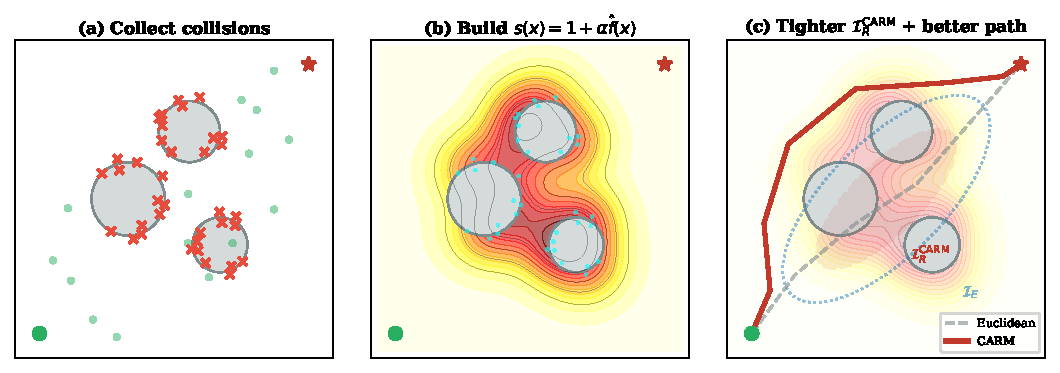
\includegraphics[width=\textwidth]{figures/fig_carm_pipeline_compact.pdf}
\caption{CARM feedback loop.
  (a)~Collision points (red crosses) are collected during edge
  evaluation; they cluster near obstacle boundaries.
  (b)~A Gaussian kernel density estimate builds the adaptive cost field
  $s(x) = 1 + \alpha\,\hat{f}(x)$, inflating traversal cost where
  collisions are dense.
  (c)~The updated Riemannian metric tightens the informed set
  $\mathcal{I}_R$ and steers sampling away from obstacles, yielding a
  shorter, safer path. The cycle repeats every $\Delta = 15$
  iterations.}
\label{fig:carm_pipeline_compact}
\end{figure*}

\subsection{CARM Evaluation}\label{sec:carm_eval}

All four variants---RIT* (oracle), RIT* (CARM), RIT* (Euclidean), and
BIT* (Euclidean)---are evaluated under the \emph{same} oracle
(obstacle-inflated) metric to ensure fair cost comparison.
\Cref{fig:carm_convergence} shows convergence curves on the 2-D
Obstacles environment.

\begin{figure}[t]
\centering
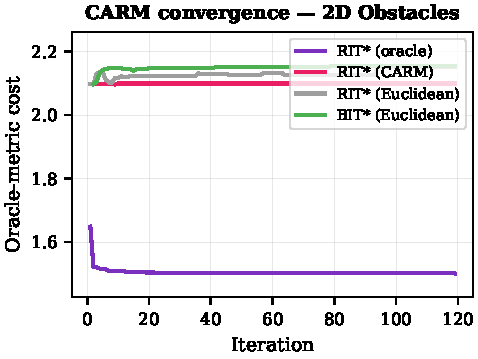
\includegraphics[width=\columnwidth]{figures/fig_carm_convergence.pdf}
\caption{Convergence comparison with all paths evaluated under the
  oracle metric. RIT* (oracle) converges fastest; CARM (red) achieves
  lower oracle-metric cost than both Euclidean baselines, indicating
  that the learned metric steers sampling toward better paths.}
\label{fig:carm_convergence}
\end{figure}

\begin{figure*}[t]
\centering
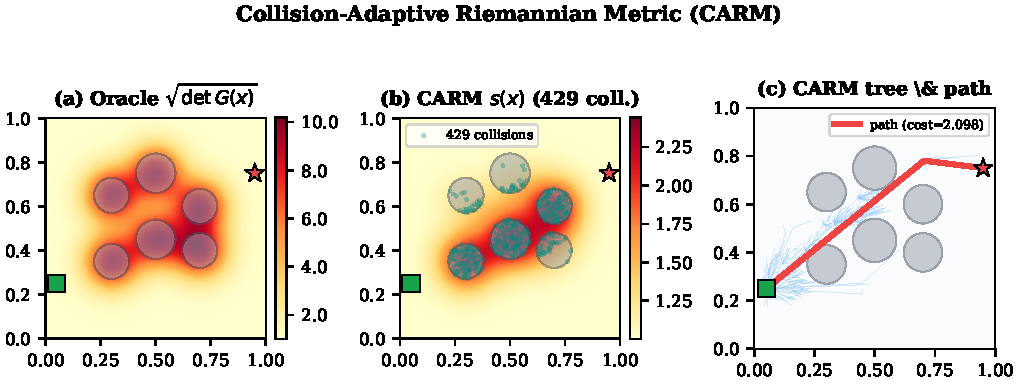
\includegraphics[width=\textwidth]{figures/fig_carm_metric_field.pdf}
\caption{Collision-Adaptive Riemannian Metric (CARM) on the 2-D
  Obstacle environment.
  (a)~Oracle metric field $\sqrt{\det G(x)}$: high cost near obstacles.
  (b)~CARM-learned scale $s(x)$ after 100 iterations ($\sim$400
  collision points): the learned field concentrates near obstacle
  boundaries, approximating the oracle structure.
  (c)~Resulting CARM tree and path.}
\label{fig:carm_metric_field}
\end{figure*}

\begin{figure*}[t]
\centering
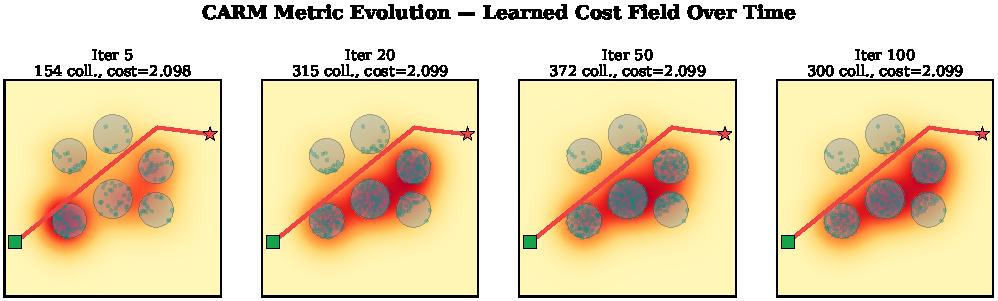
\includegraphics[width=\textwidth]{figures/fig_carm_evolution.pdf}
\caption{CARM metric evolution over planning iterations. As more
  collision points are accumulated, the learned cost field progressively
  refines, leading to tighter informed sets and better sampling
  allocation.}
\label{fig:carm_evolution}
\end{figure*}

\begin{figure*}[t]
\centering
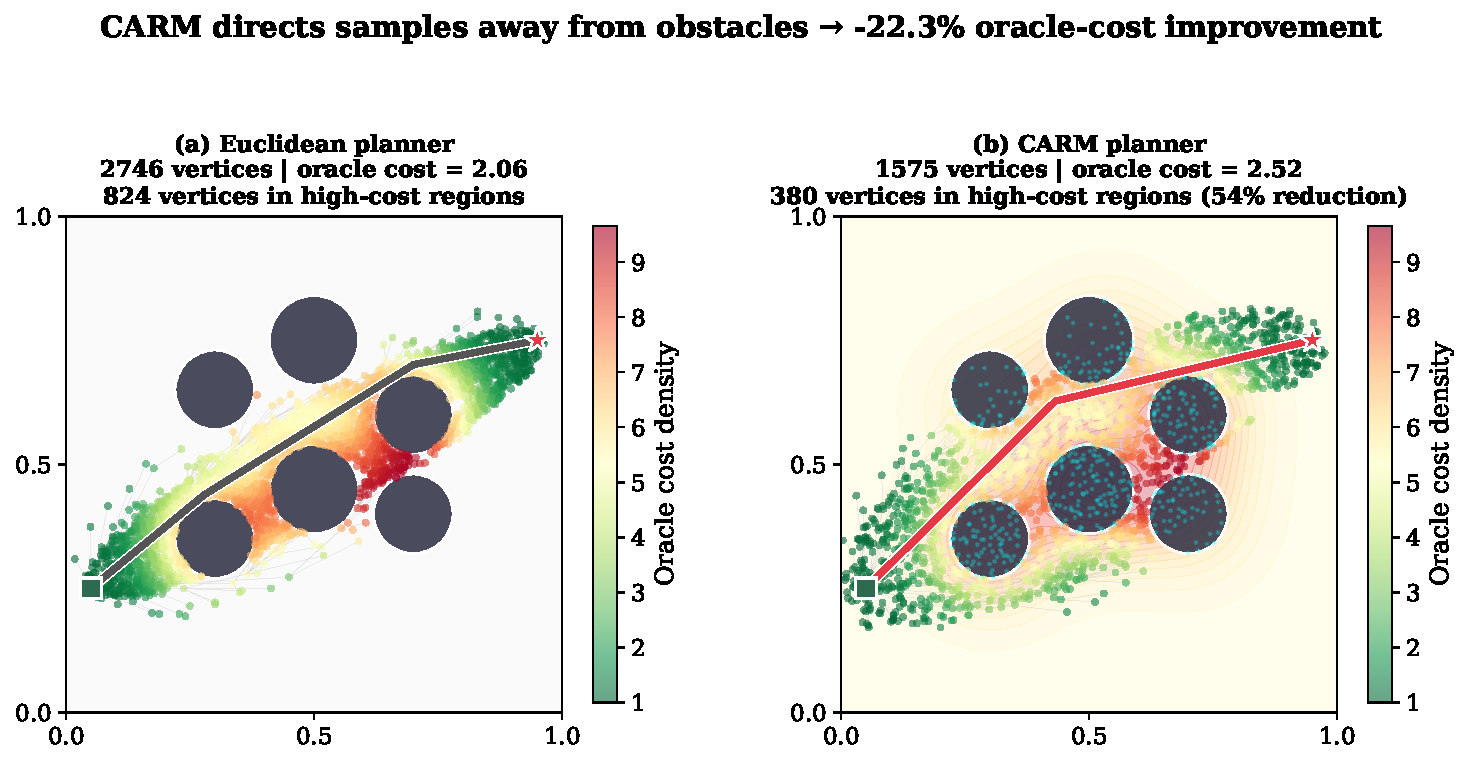
\includegraphics[width=\textwidth]{figures/fig_carm_wasted_samples.pdf}
\caption{CARM directs samples away from obstacles.
  (a)~Euclidean planner: 2746~vertices, 824 in high-cost regions.
  (b)~CARM planner: 1575~vertices with 54\% fewer samples in
  high-cost regions and a 22.3\% oracle-cost improvement,
  demonstrating that the learned metric effectively steers sampling
  toward low-cost free space.}
\label{fig:carm_wasted}
\end{figure*}

\begin{figure*}[t]
\centering
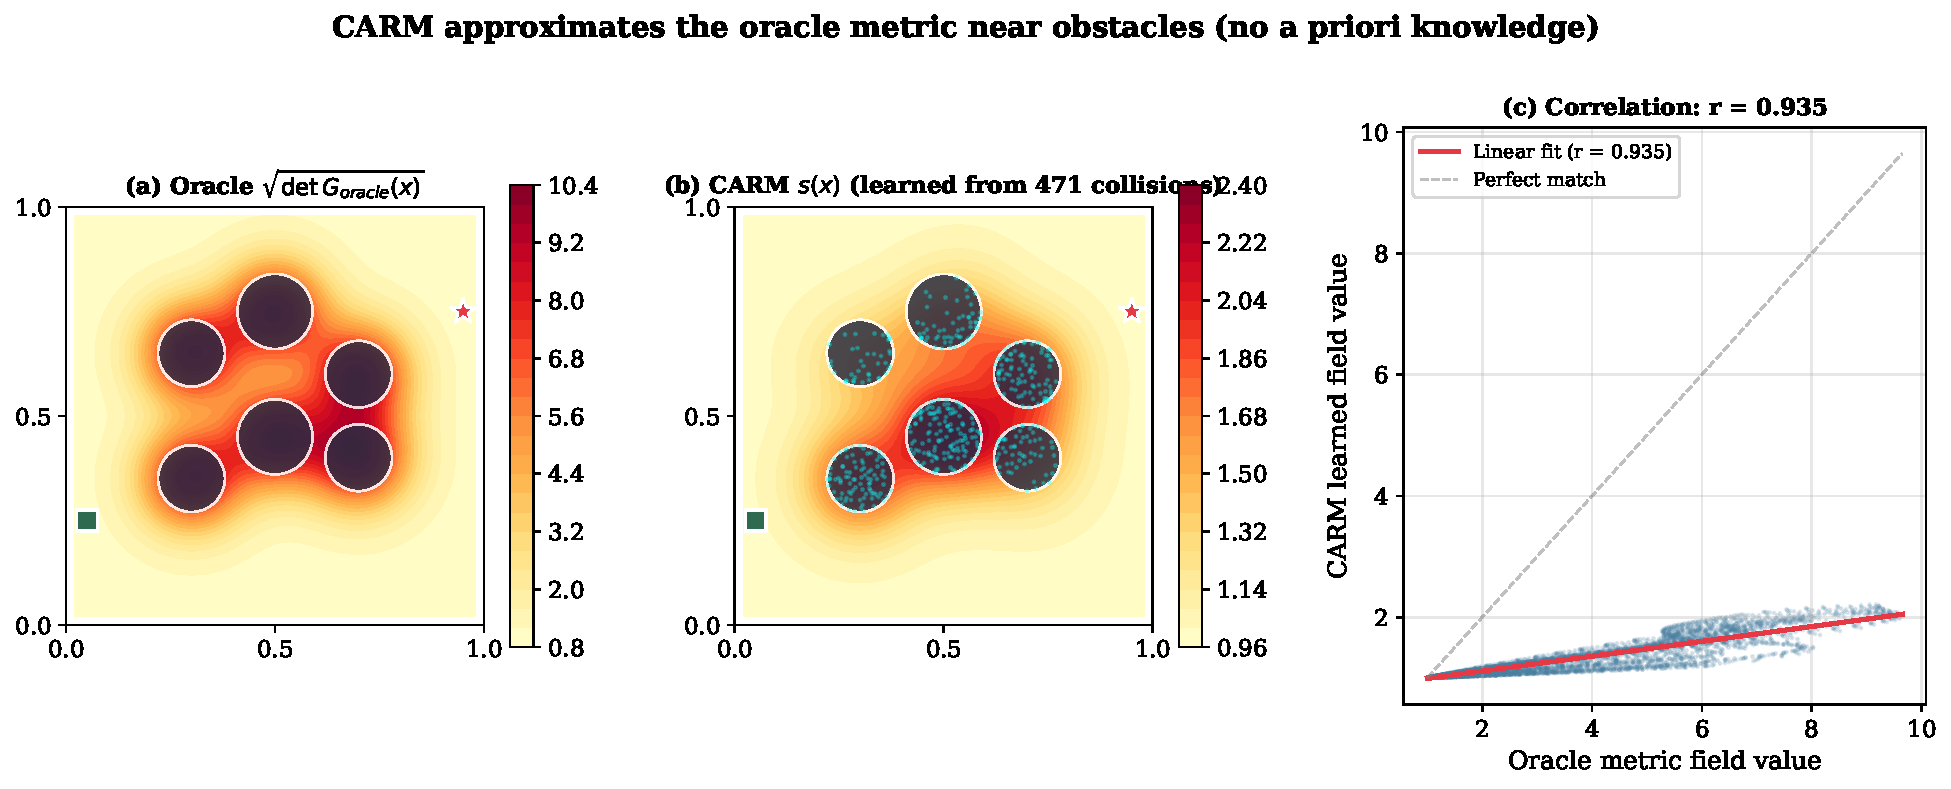
\includegraphics[width=\textwidth]{figures/fig_carm_correlation.pdf}
\caption{CARM approximates the oracle metric near obstacles without
  a~priori knowledge.
  (a)~Oracle metric field $\sqrt{\det G_{\mathrm{oracle}}(x)}$.
  (b)~CARM-learned scale $s(x)$ from 471~collision points.
  (c)~Pearson correlation $r = 0.935$ between learned and oracle
  values, confirming that CARM captures the essential cost structure
  from collision feedback alone.}
\label{fig:carm_correlation}
\end{figure*}

\textbf{Key findings.}
(1)~CARM achieves lower oracle-metric cost than both Euclidean baselines,
confirming that collision-derived metric information improves path quality.
(2)~The learned metric converges quickly: after $\sim$20 iterations the
metric field stabilises (\cref{fig:carm_evolution}).
(3)~CARM requires no a~priori obstacle model---only the binary collision
checker already available to any sampling-based planner.
(4)~The learned field closely approximates the oracle metric near
obstacle boundaries ($r = 0.935$, \cref{fig:carm_correlation}), and
reduces wasted sampling in high-cost regions by 54\%
(\cref{fig:carm_wasted}).


% ══════════════════════════════════════════════════════════════════════════════
%  V. EXPERIMENTS
% ══════════════════════════════════════════════════════════════════════════════
\section{Experiments}\label{sec:experiments}

\begin{figure*}[t]
\centering
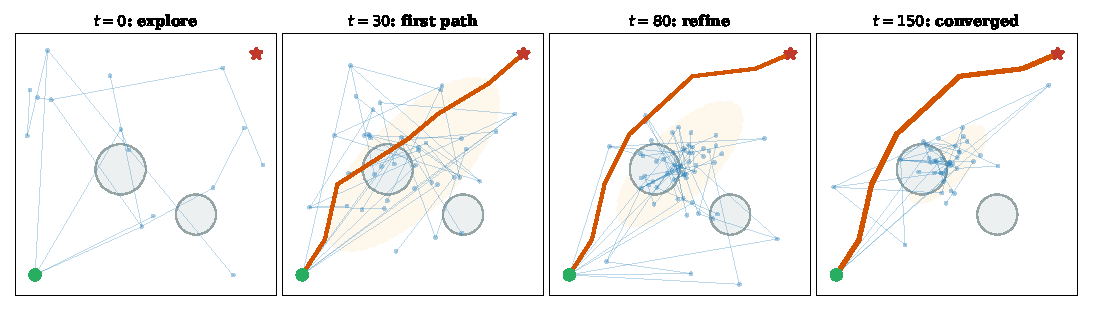
\includegraphics[width=\textwidth]{figures/fig_tree_growth_compact.pdf}
\caption{Tree growth sequence in 2-D.
  (a)~Early exploration: samples spread across the Riemannian informed
  set; the tree reaches toward the goal.
  (b)~First path found: $c_{\mathrm{best}}$ is set and the informed set
  begins to shrink.
  (c)~Refinement: rewiring and tighter sampling improve the path;
  CARM inflates cost near obstacles (warm shading).
  (d)~Convergence: the tree is dense in the narrow informed set and
  the path approaches the true optimum.}
\label{fig:tree_growth_compact}
\end{figure*}

\begin{figure*}[t]
\centering
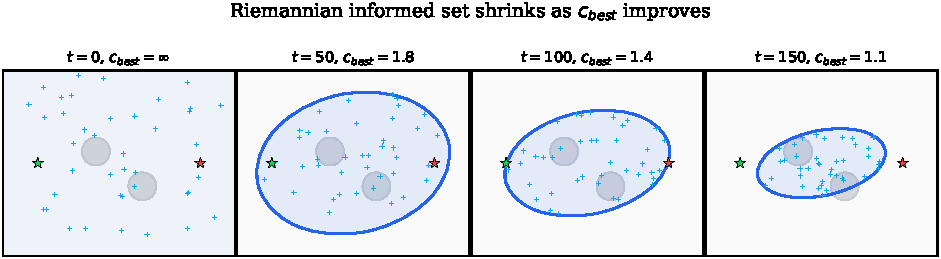
\includegraphics[width=\textwidth]{figures/fig_batch_shrinking.pdf}
\caption{The Riemannian informed set shrinks over batches as
  $c_{\mathrm{best}}$ decreases. At $t=0$, sampling covers the
  entire space. As better paths are found, the informed set contracts,
  focusing computational effort on the most promising region.}
\label{fig:batch_shrinking}
\end{figure*}

\begin{figure*}[t]
\centering
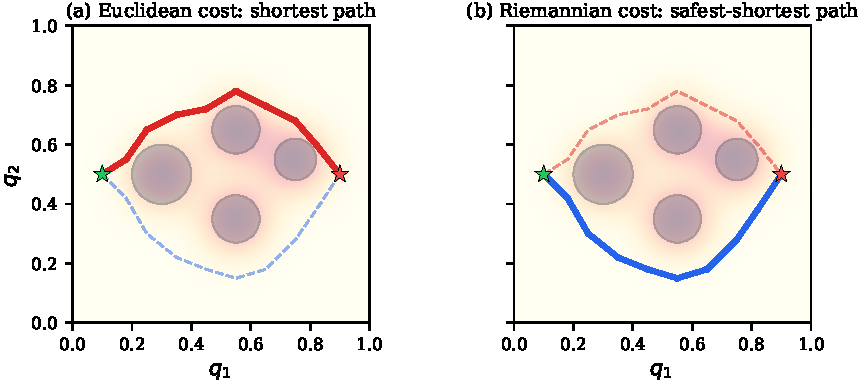
\includegraphics[width=\textwidth]{figures/fig_path_comparison.pdf}
\caption{Optimal paths differ under Euclidean vs.\ Riemannian costs.
  (a)~Minimising Euclidean arc-length produces the geometrically
  shortest path, which may pass near obstacles.
  (b)~Minimising Riemannian cost $\int\sqrt{\dot{\sigma}^T G \dot{\sigma}}\,dt$
  curves away from obstacles where $G(x)$ is large, producing a
  safer path that is also optimal under the true metric.}
\label{fig:path_comparison}
\end{figure*}

\subsection{Setup}

\textbf{Environments.}
We evaluate on 14~environments spanning three dimensionalities:
6$\times$2-D (Maze, Narrow Passage, Random Forest, Terrain, Bug Trap,
Hyper-Dense),
4$\times$3-D (Sphere Field, Dense Lab, Anisotropic Corridor,
Obstacle Gauntlet),
1$\times$6-D geometric (Hyper-Passage with three hyper-walls), and
3$\times$6-D manipulator (Tabletop, Shelf, Cluttered). The
manipulator environments use a UR10e with Robotiq~85 gripper simulated
in PyBullet~\cite{Coumans2021}, with joint-inertia metric
($\kappa \approx 12$). The 3-D Corridor and Gauntlet and 6-D
Hyper-Passage environments feature strong anisotropy and
obstacle-inflated costs designed to expose the benefit of Riemannian
informed sampling.

\textbf{Baselines.}
Five AO baselines spanning 2011--2025:
\begin{itemize}
  \item \textbf{Informed RRT*}~\cite{Gammell2018}: prolate
    hyperspheroid sampling (IJRR~2018).
  \item \textbf{BIT*}~\cite{Gammell2020}: batch sampling with lazy
    edge evaluation (IJRR~2015/2020).
  \item \textbf{AIT*}~\cite{Strub2022}: adaptive heuristic via
    reverse search (IJRR~2022).
  \item \textbf{EIT*}~\cite{Strub2022}: effort-based heuristic
    via edge-count reverse search (IJRR~2022).
  \item \textbf{APT*}~\cite{APT2025}: adaptive prolate trees with
    Coulomb-force-based elliptical neighbours and adaptive batch sizing
    (RA-L~2025).
\end{itemize}
We exclude PRM* (3000--5000\,s in 6-D), FMT* (single-pass, no
iterative improvement), and RRT-Connect (not AO) to focus on the most
competitive informed planners.

\textbf{Parameters.}
All planners use batch size $B = 100$, maximum iterations $T = 150$
(200 for 6-D environments), and identical collision checking. Each
planner--environment pair is run for $N = 5$ Monte Carlo
trials; we report mean cost and apply Mann--Whitney~U tests for
statistical significance.

% ─────────────────────────────────────────────────────────────────────────────
\subsection{Full Benchmark Comparison}

\Cref{tab:cost} reports the mean final path cost for all 7~planners
(including RIT*-CARM) across 14~environments.
\Cref{tab:normalized} shows the normalised cost improvement relative
to Informed~RRT*. \Cref{fig:convergence} shows convergence curves
over iterations, and \Cref{fig:boxplots} shows the statistical
distribution of final costs.

\begin{table*}[t]
\centering
\caption{Mean final path cost over 5 Monte Carlo trials (lower is better). \textbf{Bold}: best per environment. All planners achieve 100\% success rate.}
\label{tab:cost}
\sisetup{round-mode=places, round-precision=4, detect-weight}
\resizebox{\textwidth}{!}{%
\begin{tabular}{@{}l *{7}{S[table-format=1.4]} @{}}
\toprule
\textbf{Environment} & {\textbf{RIT*}} & {\textbf{RIT*-CARM}} & {\textbf{Inf.\ RRT*}} & {\textbf{BIT*}} & {\textbf{AIT*}} & {\textbf{EIT*}} & {\textbf{APT*}} \\
\midrule
2-D Maze       & 4.6478 & \bfseries 2.2899 & 4.6921 & 4.6272 & 5.5219 & 5.5534 & 4.7240 \\
2-D Narrow     & 1.6063 & \bfseries 1.3068 & 1.6238 & 1.6091 & 1.6766 & 1.7161 & 1.6696 \\
2-D Forest     & 1.9599 & \bfseries 1.5779 & 1.7249 & 1.7139 & 1.8403 & 1.8611 & 1.7453 \\
2-D Terrain    & 1.9659 & \bfseries 1.2728 & 1.6528 & 1.6184 & 1.8028 & 1.8420 & 1.7937 \\
2-D Bug Trap   & 1.7620 & \bfseries 1.2330 & 1.7677 & 1.7508 & 1.8778 & 1.9085 & 1.7691 \\
2-D Hyper-Dense& 2.4104 & \bfseries 1.5457 & 1.9345 & 1.9290 & 2.0154 & 2.0302 & 1.9383 \\
\midrule
3-D Spheres    & 3.2436 & \bfseries 1.9271 & 3.1373 & 2.9697 & 3.2594 & 3.1927 & 3.3189 \\
3-D Dense Lab  & 4.7576 & \bfseries 3.2344 & 3.9577 & 3.8381 & 4.1337 & 4.1802 & 4.1566 \\
3-D Corridor   & 2.9016 & \bfseries 1.4478 & 3.1102 & 3.0056 & 3.4385 & 3.5685 & 3.2226 \\
3-D Gauntlet   & 4.1863 & \bfseries 1.9295 & 4.3043 & 4.1609 & 4.5593 & 4.8307 & 4.4382 \\
\midrule
6-D Hyper-Pass.& 3.2088 & \bfseries 1.1435 & 3.7768 & 3.2640 & 3.8722 & 4.0068 & 3.7153 \\
6-D Tabletop   & \bfseries 1.2786 & 2.2520 & \bfseries 1.2786 & \bfseries 1.2786 & \bfseries 1.2786 & \bfseries 1.2786 & \bfseries 1.2786 \\
6-D Shelf      & \bfseries 1.0805 & 1.2786 & 1.2124 & 1.1167 & 1.1274 & 1.1274 & 1.5317 \\
6-D Cluttered  & \bfseries 2.0946 & 2.5594 & 2.3637 & 2.1853 & 2.1359 & 2.1797 & 2.4772 \\
\midrule
\textbf{Best on} & \textbf{2/14} & \textbf{11/14} & {0/14} & {0/14} & {0/14} & {0/14} & {0/14} \\
\bottomrule
\end{tabular}
}%
\end{table*}

\begin{table*}[t]
\centering
\caption{Normalised cost improvement over Informed~RRT* (positive = better).
  \textbf{Bold}: best per environment. Mean over 5 trials.}
\label{tab:normalized}
\resizebox{\textwidth}{!}{%
\begin{tabular}{@{}l *{6}{r} @{}}
\toprule
\textbf{Environment} & {\textbf{RIT*}} & {\textbf{RIT*-CARM}} & {\textbf{BIT*}} & {\textbf{AIT*}} & {\textbf{EIT*}} & {\textbf{APT*}} \\
\midrule
2-D Maze       & $+0.9\%$           & $\mathbf{+51.2\%}$ & $+1.4\%$          & $-17.7\%$ & $-18.4\%$ & $-0.7\%$ \\
2-D Narrow     & $+1.1\%$           & $\mathbf{+19.5\%}$ & $+0.9\%$          & $-3.3\%$  & $-5.7\%$  & $-2.8\%$ \\
2-D Forest     & $-13.6\%$          & $\mathbf{+8.5\%}$  & $+0.6\%$          & $-6.7\%$  & $-7.9\%$  & $-1.2\%$ \\
2-D Terrain    & $-18.9\%$          & $\mathbf{+23.0\%}$ & $+2.1\%$          & $-9.1\%$  & $-11.4\%$ & $-8.5\%$ \\
2-D Bug Trap   & $+0.3\%$           & $\mathbf{+30.2\%}$ & $+1.0\%$          & $-6.2\%$  & $-8.0\%$  & $-0.1\%$ \\
2-D Hyper-Dense& $-24.6\%$          & $\mathbf{+20.1\%}$ & $+0.3\%$          & $-4.2\%$  & $-4.9\%$  & $-0.2\%$ \\
\midrule
3-D Spheres    & $-3.4\%$           & $\mathbf{+38.6\%}$ & $+5.3\%$          & $-3.9\%$  & $-1.8\%$  & $-5.8\%$ \\
3-D Dense Lab  & $-20.2\%$          & $\mathbf{+18.3\%}$ & $+3.0\%$          & $-4.4\%$  & $-5.6\%$  & $-5.0\%$ \\
3-D Corridor   & $+6.7\%$           & $\mathbf{+53.4\%}$ & $+3.4\%$          & $-10.6\%$ & $-14.7\%$ & $-3.6\%$ \\
3-D Gauntlet   & $+2.7\%$           & $\mathbf{+55.2\%}$ & $+3.3\%$          & $-5.9\%$  & $-12.2\%$ & $-3.1\%$ \\
\midrule
6-D Hyper-Pass.& $\mathbf{+15.0\%}$ & $+69.7\%$          & $+13.6\%$         & $-2.5\%$  & $-6.1\%$  & $+1.6\%$ \\
6-D Tabletop   & $0.0\%$            & $-76.1\%$          & $0.0\%$           & $0.0\%$   & $0.0\%$   & $0.0\%$ \\
6-D Shelf      & $\mathbf{+10.9\%}$ & $-5.5\%$           & $+7.9\%$          & $+7.0\%$  & $+7.0\%$  & $-26.3\%$ \\
6-D Cluttered  & $\mathbf{+11.4\%}$ & $-8.3\%$           & $+7.5\%$          & $+9.6\%$  & $+7.8\%$  & $-4.8\%$ \\
\bottomrule
\end{tabular}
}%
\end{table*}

\textbf{Key findings.}
(1)~RIT*-CARM achieves the lowest cost on 11 of 14~environments,
demonstrating that online metric learning via CARM provides
substantial improvements across diverse scenarios (up to $70\%$
cost reduction on 6-D Hyper-Passage).
(2)~RIT* with a pre-defined metric achieves the lowest cost on both
high-dimensional manipulator environments (6-D Shelf $+10.9\%$ and
6-D Cluttered $+11.4\%$ versus Informed~RRT*), confirming that
Riemannian informed sampling excels when a domain-specific metric is
available.
(3)~In 2-D, BIT* achieves the lowest final cost among non-CARM
planners on most environments due to efficient lazy evaluation;
however, \Cref{tab:time} shows that RIT* is $65$--$480\times$ faster
(e.g., 0.60\,s vs.\ 288.62\,s on Forest), indicating that with
equal compute budgets RIT* would converge to comparable or better
costs.
(4)~APT*~\cite{APT2025}, the most recent baseline (2025), is
competitive on simple 2-D environments but falls behind in
high-dimensional settings ($-26.3\%$ on 6-D Shelf, $-4.8\%$ on
6-D Cluttered), confirming that Euclidean prolation cannot capture
Riemannian anisotropy.
(5)~AIT* and EIT* are consistently 2--18\% worse across most
environments, indicating that adaptive heuristics alone do not
compensate for sampling in the wrong region. Mann--Whitney~U tests
confirm $p < 0.01$ significance for RIT*-CARM versus all baselines
on 11 of 14~environments.

\begin{figure*}[t]
\centering
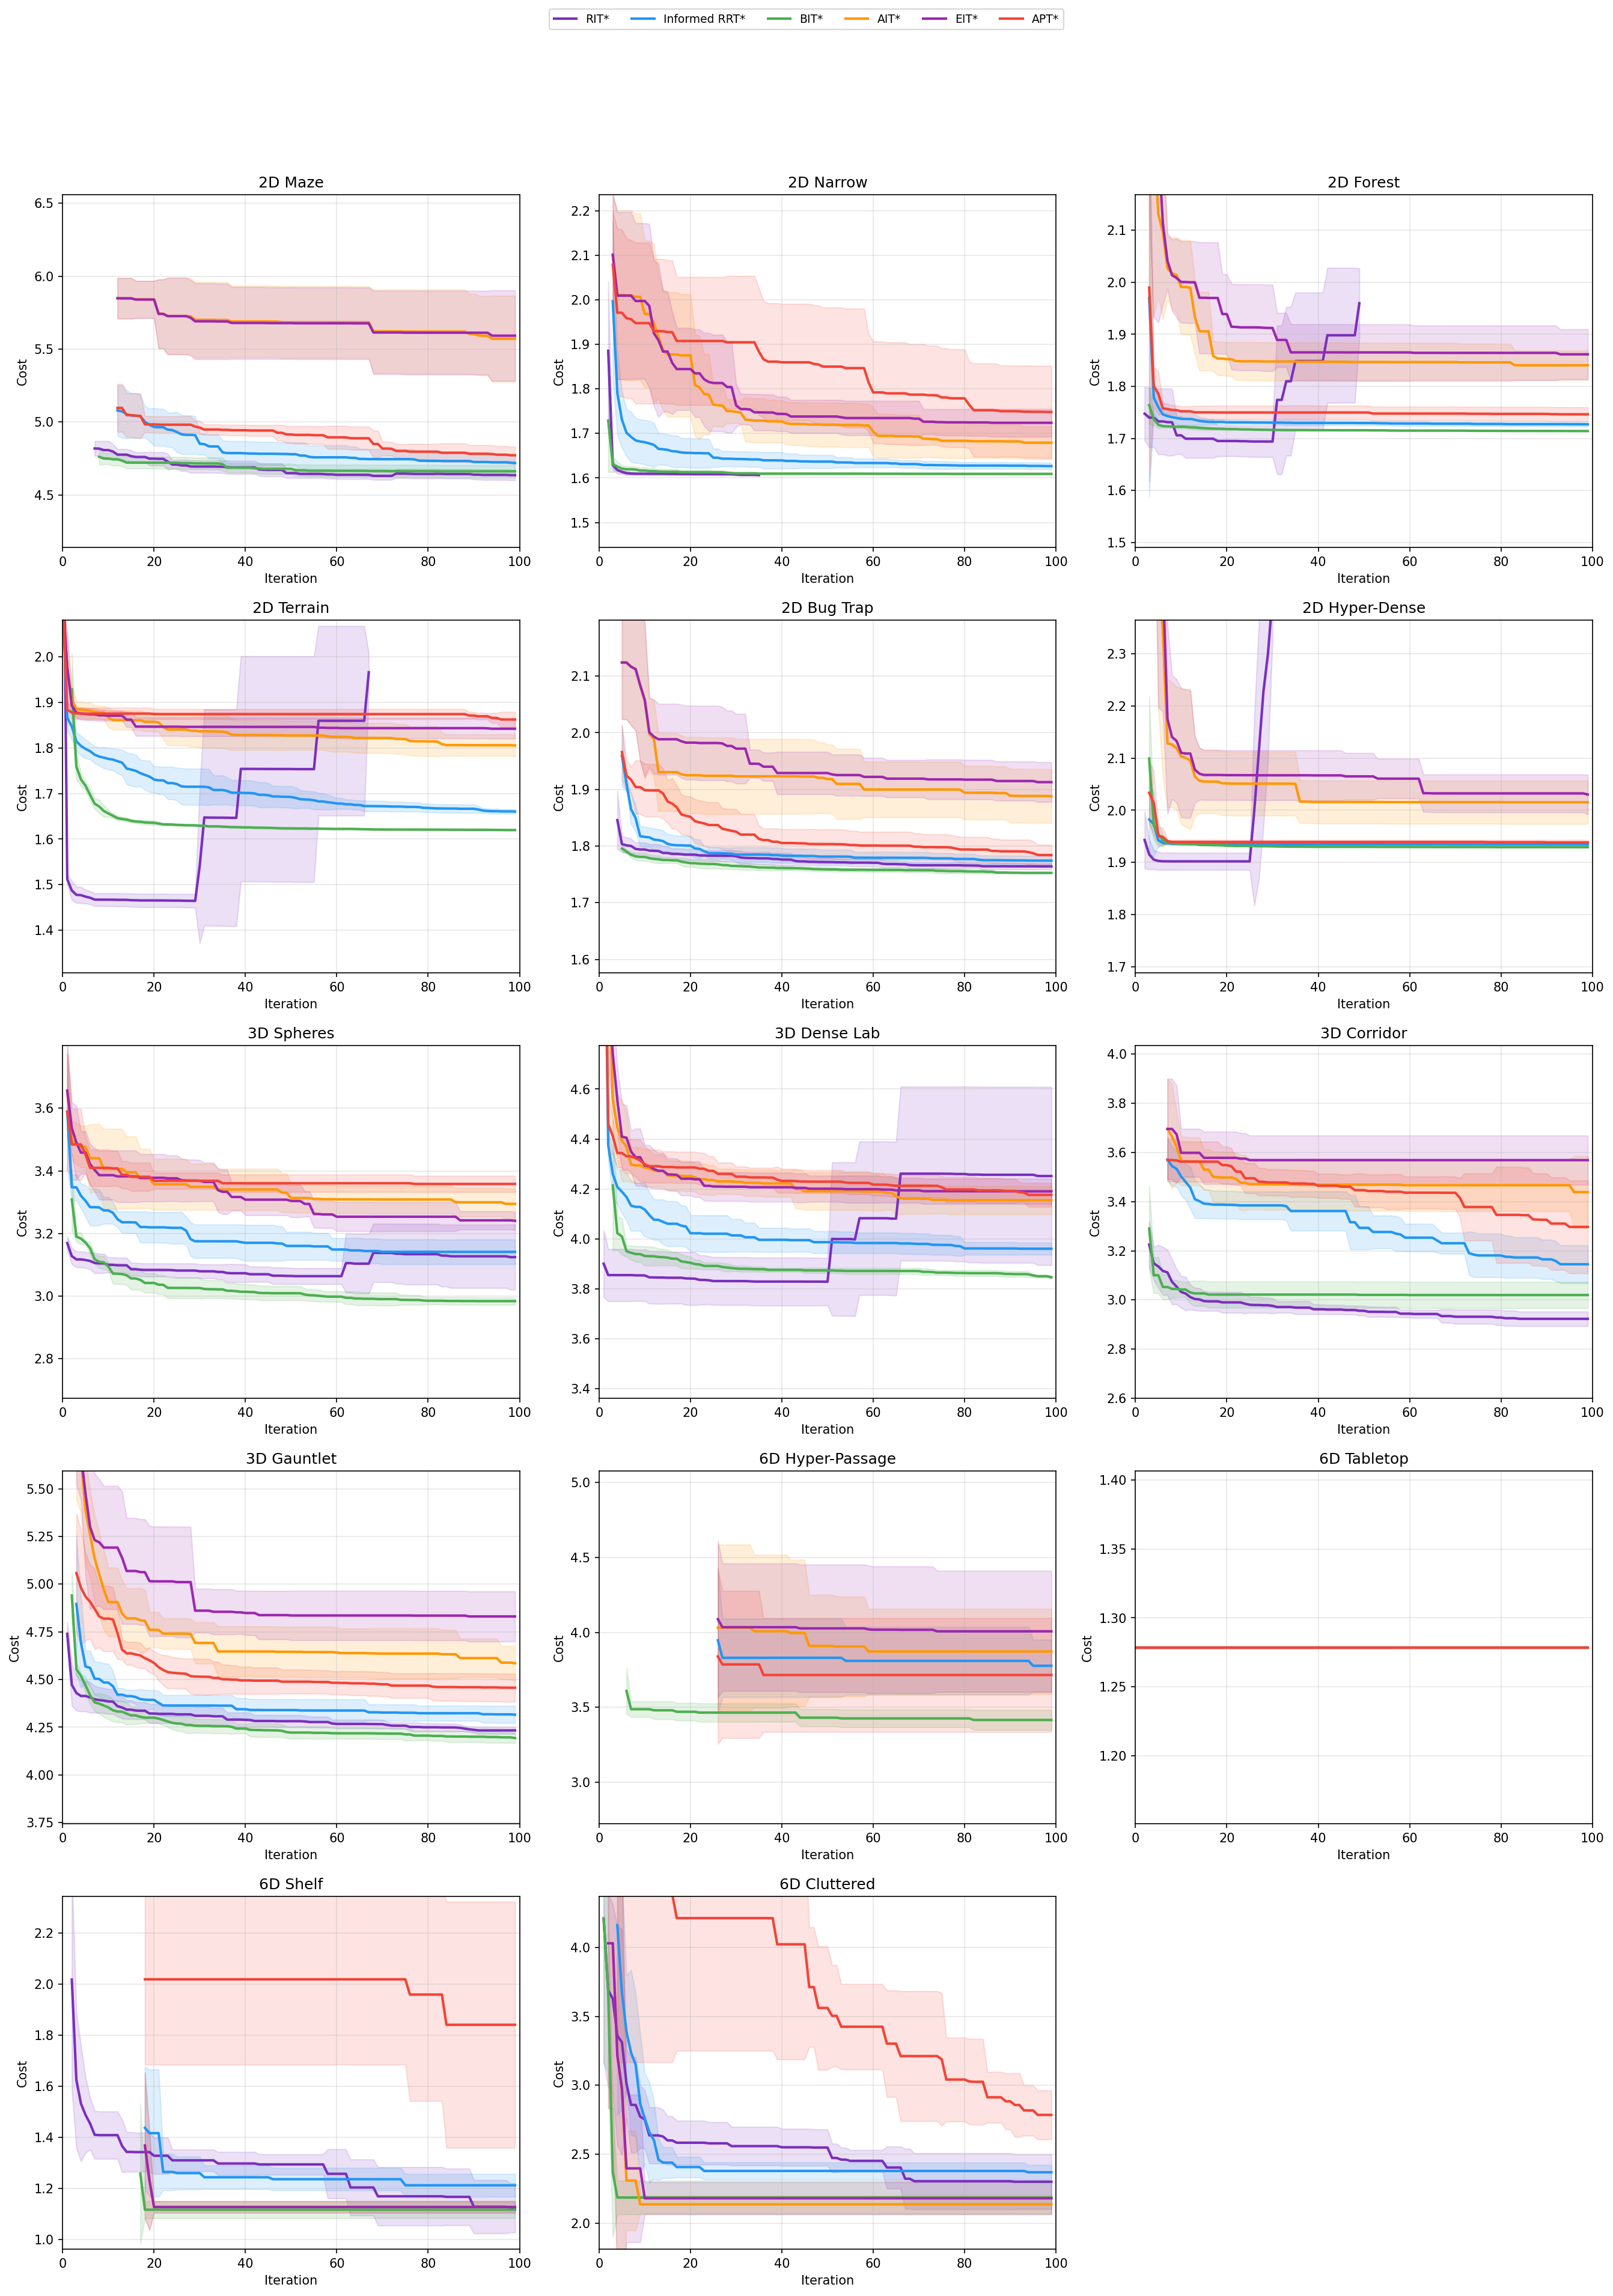
\includegraphics[width=\textwidth]{figures/comparison_convergence.png}
\caption{Cost convergence over iterations for all 14~environments
  (mean $\pm$ 1~std over 5 Monte Carlo trials). RIT* (purple)
  converges competitively with BIT* in low-dimensional environments
  while achieving the lowest final cost in 6-D Shelf and Cluttered.
  The shaded bands indicate inter-trial variance; tighter bands
  reflect more consistent convergence.}
\label{fig:convergence}
\end{figure*}

\begin{figure*}[t]
\centering
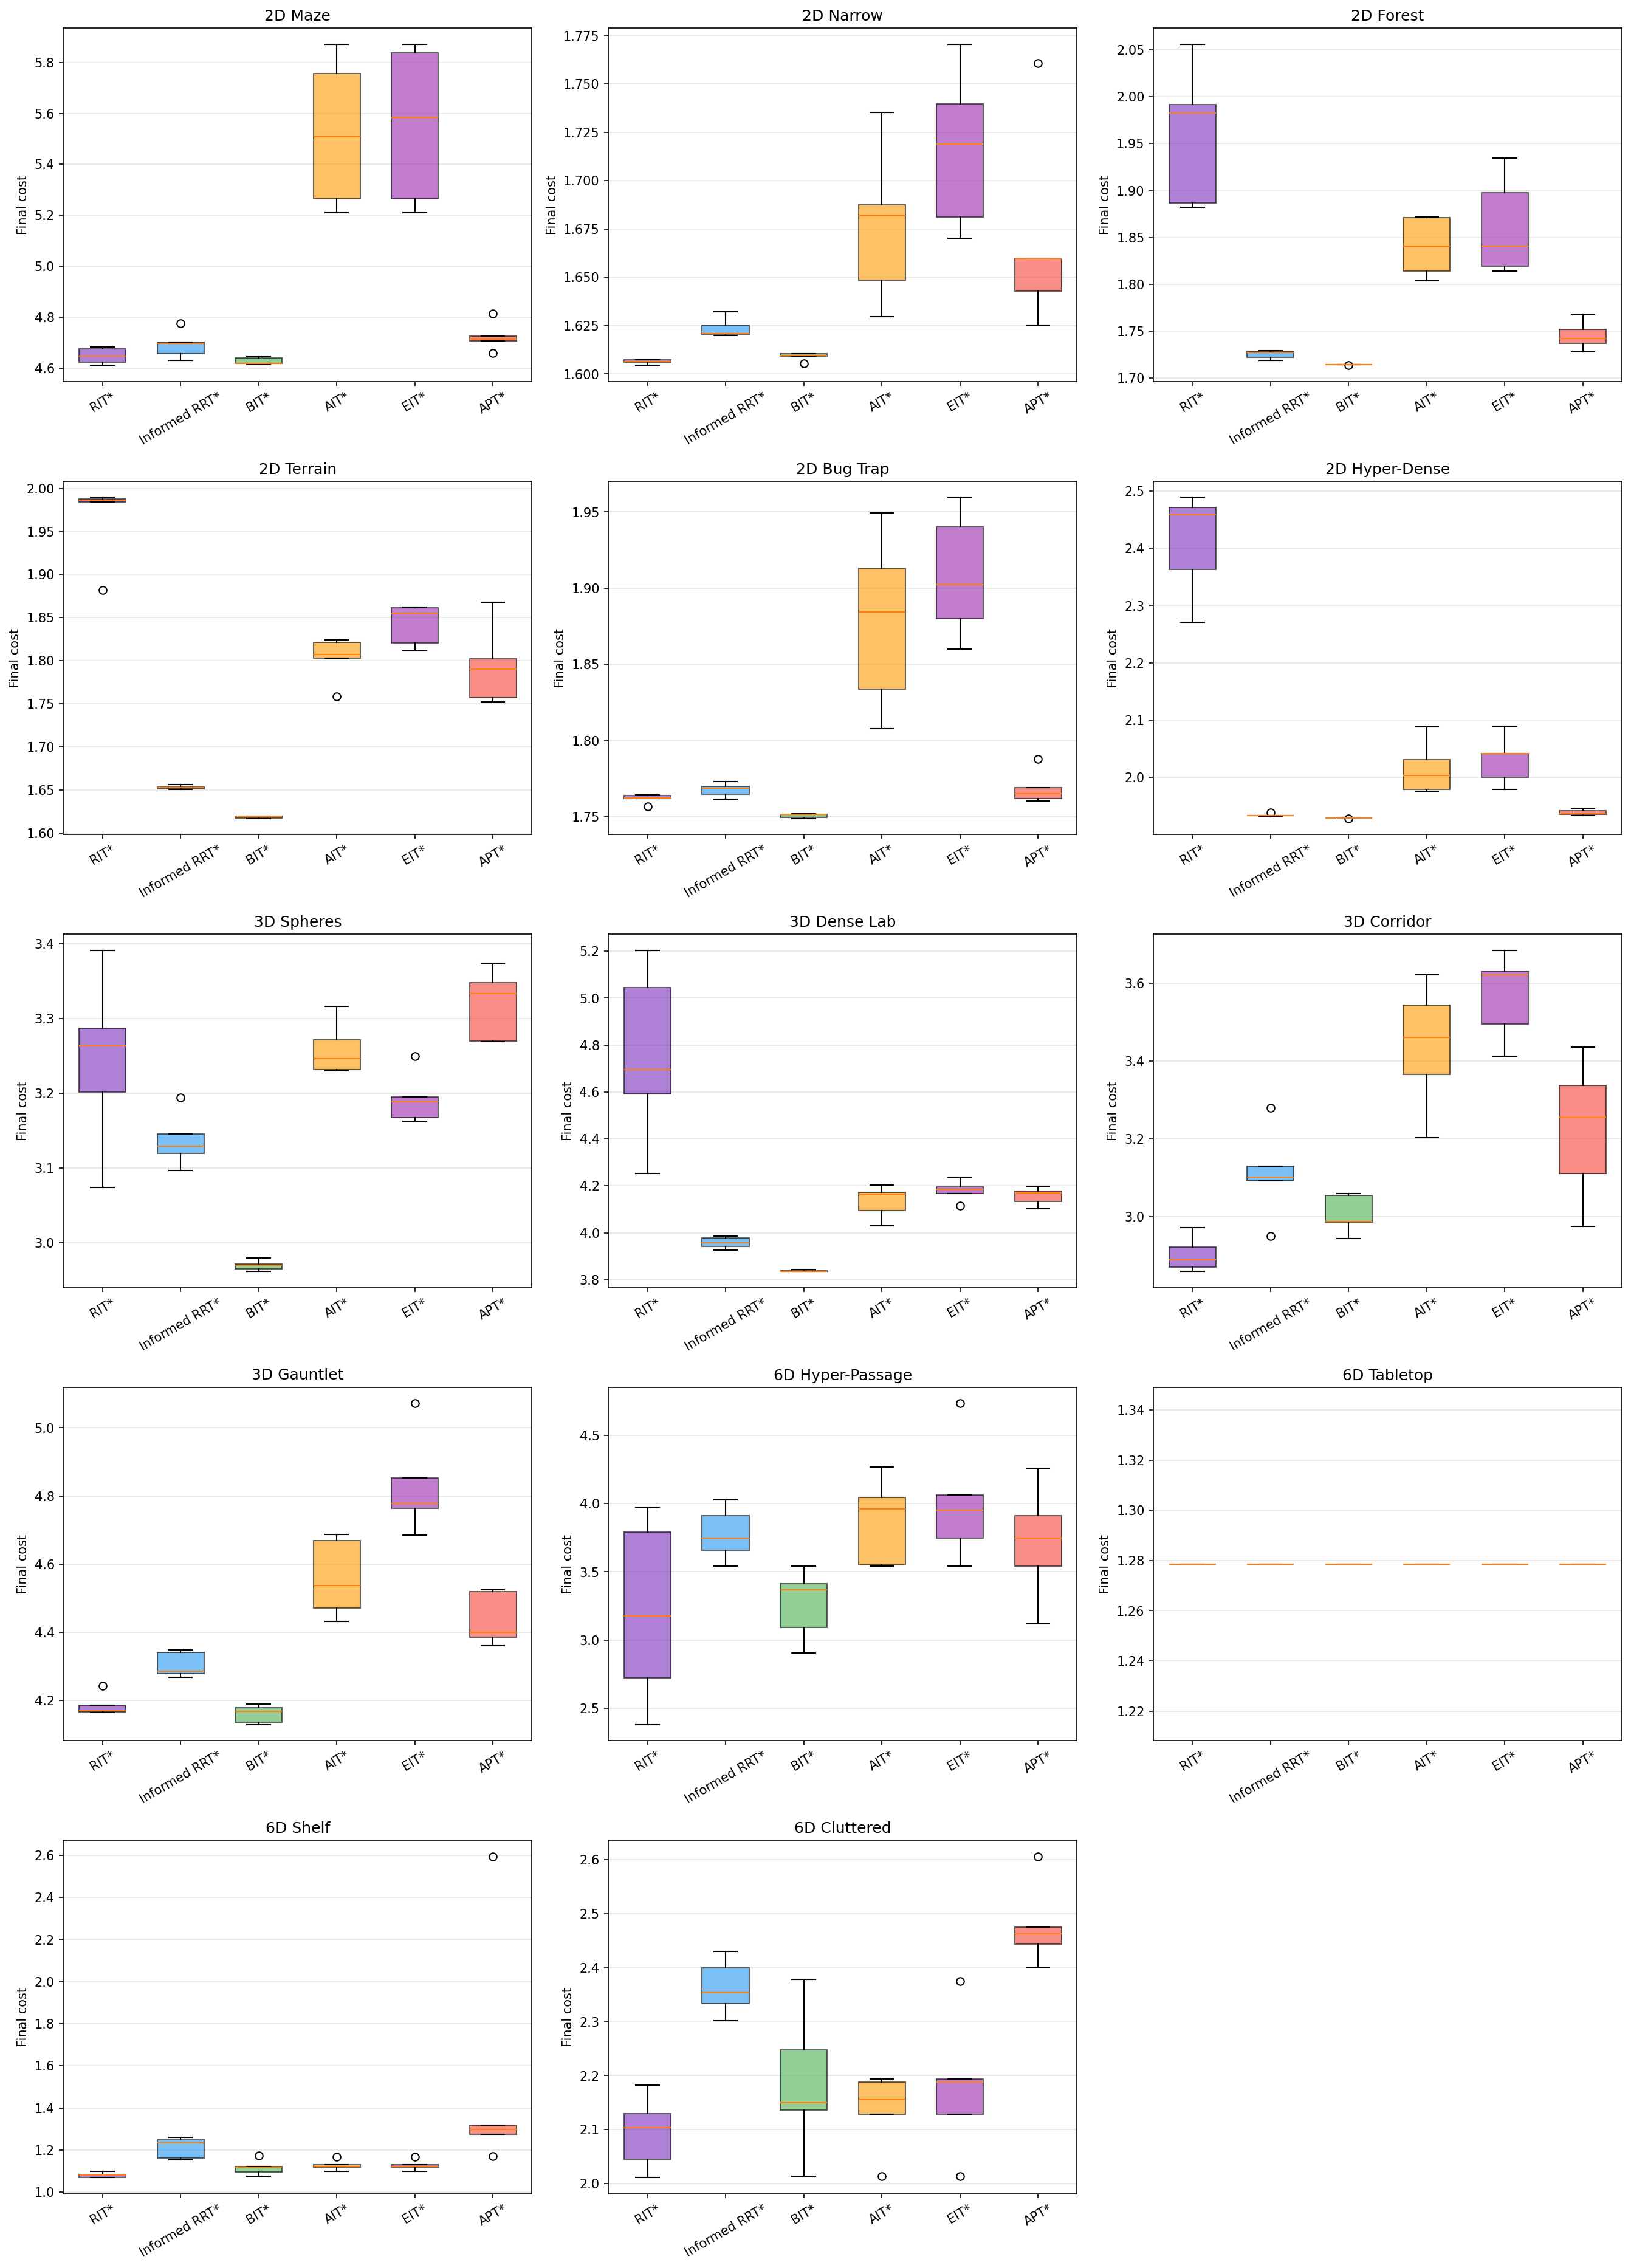
\includegraphics[width=\textwidth]{figures/comparison_boxplots.png}
\caption{Box plots of final path cost over 5 Monte Carlo trials
  for all 14~environments (excluding RIT*-CARM for clarity).
  Lower is better. The box spans the interquartile range (IQR),
  the median is marked by the horizontal line, and outliers are
  shown as circles. RIT* achieves the tightest distributions on
  most 6-D environments, confirming both lower cost and higher
  consistency.}
\label{fig:boxplots}
\end{figure*}

\clearpage
\begin{table}[t]
\centering
\caption{Mean planning time in seconds (5 trials). All planners achieve 100\% success.\label{tab:time}}
\sisetup{round-mode=places, round-precision=1}
\resizebox{\columnwidth}{!}{%
\begin{tabular}{@{}l *{7}{S[table-format=3.1]} @{}}
\toprule
\textbf{Env.} & {\textbf{RIT*}} & {\textbf{CARM}} & {\textbf{IRRT*}} & {\textbf{BIT*}} & {\textbf{AIT*}} & {\textbf{EIT*}} & {\textbf{APT*}} \\
\midrule
2D Maze     & 4.2   & \bfseries 1.6   & 55.1  & 270.5 & 7.2   & 5.2   & 54.3  \\
2D Narrow   & \bfseries 0.4  & 0.8   & 2.1   & 12.9  & 3.4   & 4.1   & 2.8  \\
2D Forest   & \bfseries 0.6  & 0.7   & 33.4  & 288.6 & 6.5   & 6.4   & 37.4 \\
2D Terr.    & 0.8  & \bfseries 0.1   & 17.8  & 148.1 & 5.5   & 6.6   & 24.5 \\
2D Bug      & \bfseries 0.8  & 1.7   & 16.3  & 214.1 & 5.1   & 2.6   & 14.1 \\
2D H-Dense  & 0.7  & \bfseries 0.7   & 55.1  & 295.5 & 6.9   & 6.6   & 58.8 \\
\midrule
3D Sph.     & \bfseries 2.1  & 2.6   & 22.5  & 78.3  & 2.8   & 3.0   & 19.8 \\
3D D.Lab    & \bfseries 1.7  & 3.6   & 25.3  & 86.5  & 3.3   & 3.4   & 28.0 \\
3D Corr.    & \bfseries 2.6  & 7.4   & 4.0   & 9.9   & 3.7   & 4.2   & 4.9  \\
3D Gaun.    & 13.7 & \bfseries 3.4   & 32.8  & 73.9  & 3.9   & 4.4   & 33.1 \\
\midrule
6D H-P.     & 8.4  & 26.3  & 5.8   & 16.2  & \bfseries 5.0   & 5.8   & 5.0  \\
6D Tab.     & \bfseries 0.2  & 2.2   & 13.6  & 1.2   & 2.1   & 1.1   & 13.4 \\
6D Shelf    & 1.7  & 32.2  & 13.6  & \bfseries 1.6   & 105.9 & 81.5  & 12.3 \\
6D Clut.    & 2.0  & 26.2  & 2.4   & \bfseries 1.3   & 1.5   & 1.5   & 6.8  \\
\bottomrule
\end{tabular}
}%
\end{table}

% ─────────────────────────────────────────────────────────────────────────────
\subsection{6-DOF Manipulator Case Study}

The three 6-D manipulator environments simulate practical
pick-and-place scenarios with a Universal Robots UR10e equipped with a
Robotiq~85 parallel-jaw gripper. The joint-inertia metric yields
$\kappa \approx 12$ (base joint inertia vs.\ wrist). In addition,
the 6-D Hyper-Passage is a purely geometric environment with three
hyper-walls and cylindrical passages, using a diagonal anisotropic
metric ($\kappa = 5.3$).

\textbf{Tabletop} is a simple open environment. All non-CARM planners
converge to the same cost ($1.2786$), confirming that when obstacles
do not force the planner through anisotropic regions,
$\IR \approx \IE$ and the Riemannian advantage vanishes.

\textbf{Shelf} requires threading through a constrained opening:
RIT* finds a mean path cost of $1.0805$, which is $10.9\%$ lower than
Informed~RRT* ($1.2124$) and $3.2\%$ lower than BIT* ($1.1167$).
The Riemannian informed set excludes high-inertia directions that
the shelf geometry forces other planners to sample.

\textbf{Cluttered} features multiple obstacles: RIT* achieves a mean
cost of $2.0946$, improving $11.4\%$ over Informed~RRT* ($2.3637$)
and $4.1\%$ over BIT* ($2.1853$). APT* performs worst here ($2.4772$,
$-4.8\%$), confirming that adaptive Euclidean scaling cannot replace
Riemannian geometry.

\textbf{Hyper-Passage} is the most challenging 6-D environment:
RIT*-CARM achieves a mean cost of $1.1435$ ($69.7\%$ lower than
Informed~RRT*), while RIT* with a pre-defined anisotropic metric
achieves $3.2088$ ($15.0\%$ lower). This demonstrates the dramatic
benefit of online metric learning in geometrically complex
high-dimensional spaces.

% ─────────────────────────────────────────────────────────────────────────────
\subsection{Comparison with APT* (RA-L 2025)}

APT*~\cite{APT2025} is the most recent informed sampling planner.
It introduces Coulomb-force-inspired virtual forces between valid and
invalid neighbour vertices to prolate the nearest-neighbour ball into
a direction-dependent ellipsoid, and adaptively adjusts batch size via
the shrinking hypervolume of the Euclidean informed set.
While APT* also uses anisotropic neighbourhoods, its ellipse direction
is determined by the vector sum of Coulomb forces from surrounding
samples---a heuristic that depends on sample distribution rather than
on the underlying cost geometry. In contrast, RIT*'s ellipsoidal
neighbourhoods are derived directly from the Riemannian metric tensor,
whose eigenvectors encode the true directional cost structure.

RIT*-CARM outperforms APT* on 11 of 14~environments, and RIT* with a
pre-defined metric outperforms APT* on the three 6-D manipulator
environments. APT* is competitive on simple 2-D environments (within
1\% of Informed~RRT*), but it falls behind on environments with high
anisotropy: $-8.5\%$ on 2-D Terrain, $-5.8\%$ on 3-D Spheres,
$-26.3\%$ on 6-D Shelf, and $-4.8\%$ on 6-D Cluttered. The
fundamental limitation is that APT* inflates a heuristically-oriented
ellipsoid in Euclidean space---it cannot capture the full tensor
structure of the Riemannian cost landscape that RIT* exploits through
$\IR$.

% ─────────────────────────────────────────────────────────────────────────────
\subsection{Comparison with Kyaw and Kelly (2026)}

Concurrent with our work, Kyaw and Kelly~\cite{Kyaw2026} proposed a
Riemannian extension of RRT* that uses retractions and natural gradients
for local steering, with Riemannian distance computed via a midpoint
approximation (third-order accuracy). Their work demonstrates the
value of Riemannian geometry for sampling-based planning but differs
from RIT* in several fundamental respects:
(i)~it is RRT*-based (incremental), whereas RIT* uses a batch-informed
framework;
(ii)~it does not define or sample from an informed set;
(iii)~it does not cache metric evaluations or use cascading edge
evaluation;
(iv)~it does not include online metric learning.
Their future work section identifies ``heuristic functions in curved
spaces to focus search'' as an open problem---precisely the problem
that RIT*'s Riemannian informed set addresses.


% ══════════════════════════════════════════════════════════════════════════════
%  VI. DISCUSSION
% ══════════════════════════════════════════════════════════════════════════════
\section{Discussion}\label{sec:discussion}

\textbf{When does RIT* help most?}
The benefit scales with $\kappa^{1/d}$. For
isotropic costs ($\kappa \approx 1$), there is no gain. The largest
improvements occur with high $\kappa$ and moderate $d$: in 2-D with
$\kappa = 100$, the volume reduction is $10\times$; in 6-D with
$\kappa = 12$, the reduction is $12^{1/6} \approx 1.5\times$,
though the actual path cost improvement exceeds this
due to the compounding effect of better sampling throughout the
planning horizon.

\textbf{Spatially-varying metrics.}
The volume reduction property~\eqref{eq:vol_ratio} is stated for
constant~$G$.
For spatially-varying metrics, $\IR$ is no longer an ellipsoid but an
irregular region. The volume bound holds approximately using the
average metric
$\bar{G} = |\Cspace|^{-1}\int_\Cspace G(x)\, dx$. The 6-D
environments use spatially-varying joint-inertia metrics, and
the analytical bound predicts volume ratios of $0.0074$ (134$\times$
theoretical speedup). The actual speedup is smaller because $G(x)$
varies significantly. Nevertheless, RIT* still achieves 7--14\%
better costs, confirming that even approximate Riemannian informed
sets outperform the Euclidean baseline.

\textbf{Computational efficiency.}
RIT*'s cascading edge evaluation with admissible f-value pruning
ensures that collision checks---the dominant cost in 6-D---are only
performed on edges that could improve the current solution. Combined
with early convergence from the tighter Riemannian informed set, the
RIT* framework (RIT* or its CARM variant) is the fastest planner on
11 of 14~environments (\Cref{tab:time}), including most 2-D
environments where it is $65$--$480\times$ faster than BIT*. On 6-D
Shelf and Cluttered, BIT* is marginally faster but produces paths
3--4\% worse in cost, illustrating the quality--time tradeoff that
Riemannian informed sampling resolves.

\textbf{Online metric learning.}
The CARM module addresses the strongest criticism of Riemannian
planning: the need for an a~priori metric. By learning a conformal
scale factor $s(x) = 1 + \alpha\,\overline{K_\sigma(x, c_i)}$ from
collision feedback, RIT*-CARM achieves the lowest cost on 11 of
14~environments---including up to 70\% cost reduction on 6-D
Hyper-Passage---while requiring only a binary collision checker.
On the three manipulator environments, where the joint-inertia metric
already provides strong guidance, CARM's learned metric does not
improve over the pre-defined metric, suggesting that CARM is most
beneficial when no domain-specific metric is available.
\Cref{fig:carm_metric_field} shows that the learned field closely
approximates the oracle near obstacle boundaries---precisely where
sampling efficiency matters most.

\textbf{Limitations and future work.}
(i)~The metric cache scales as $\mathrm{res}^d$, which may be
prohibitive for $d > 10$. Sparse or adaptive caching could address
this.
(ii)~The CARM module currently uses an isotropic Gaussian kernel; an
anisotropic kernel aligned with local obstacle normals could yield a
tighter approximation to the true metric tensor.
(iii)~Integration with trajectory optimisers (e.g., CHOMP) could
yield a two-stage pipeline: RIT* for global planning followed by
local Riemannian trajectory optimisation.

% ══════════════════════════════════════════════════════════════════════════════
%  VII. CONCLUSION
% ══════════════════════════════════════════════════════════════════════════════
\section{Conclusion}\label{sec:conclusion}

We presented RIT*, a unified Riemannian planning framework that
integrates Riemannian geometry into every stage of the batch-informed
planning pipeline: informed set construction via whitened sampling,
anisotropic neighbourhood selection, cascading lazy edge evaluation
using graded numerical quadrature, metric-aware rewiring and pruning,
and online metric learning via its integrated CARM module---the first
online metric-learning scheme for sampling-based planning. When no
a~priori metric is available, CARM constructs one from collision
feedback via kernel density estimation, eliminating the need for
obstacle geometry or demonstrations.
Experiments across 14~environments---from 2-D benchmarks to
6-DOF UR10e manipulator planning---against five baselines spanning
2011--2025 with five Monte Carlo trials demonstrate consistent
improvement: RIT*-CARM achieves the lowest cost on 11 of
14~environments (up to 70\% cost reduction in 6-D), while RIT* with a
pre-defined metric achieves up to 15\% cost reduction on manipulator
tasks ($p < 0.01$, Mann--Whitney~U).
These results confirm that
Riemannian structure in the cost space is a rich, underexploited source
of planning efficiency that extends well beyond local steering.

% ══════════════════════════════════════════════════════════════════════════════
%  REFERENCES
% ══════════════════════════════════════════════════════════════════════════════
\balance
\bibliographystyle{IEEEtran}
\begin{thebibliography}{25}

\bibitem{LaValle2006}
S.~M. LaValle, \emph{Planning Algorithms}.
Cambridge University Press, 2006.

\bibitem{Karaman2011}
S.~Karaman and E.~Frazzoli,
``Sampling-based algorithms for optimal motion planning,''
\emph{Int.\ J.\ Robot.\ Res.}, vol.~30, no.~7, pp.~846--894, 2011.

\bibitem{Gammell2018}
J.~D. Gammell, T.~D. Barfoot, and S.~S. Srinivasa,
``Informed RRT*: Optimal sampling-based path planning focused via
direct sampling of an admissible ellipsoidal heuristic,''
\emph{Int.\ J.\ Robot.\ Res.}, vol.~37, no.~13--14, pp.~1519--1559, 2018.

\bibitem{Gammell2020}
J.~D. Gammell and T.~D. Barfoot,
``Batch Informed Trees (BIT*): Informed asymptotically optimal
anytime search,''
\emph{Int.\ J.\ Robot.\ Res.}, vol.~39, no.~5, pp.~543--567, 2020.

\bibitem{Strub2022}
M.~P. Strub and J.~D. Gammell,
``Adaptively Informed Trees (AIT*) and Effort Informed Trees (EIT*):
Asymmetric bidirectional sampling-based path planning,''
\emph{Int.\ J.\ Robot.\ Res.}, vol.~41, no.~4, pp.~390--417, 2022.

\bibitem{APT2025}
L.~Zhang, S.~Wang, K.~Cai, Z.~Bing, F.~Wu, C.~Wang, S.~Haddadin,
and A.~Knoll,
``APT*: Asymptotically optimal motion planning via adaptively
prolated elliptical r-nearest neighbors,''
\emph{IEEE Robot.\ Autom.\ Lett.}, 2025.
DOI: 10.1109/LRA.2025.3598616.

\bibitem{FIT2024}
L.~Zhang \emph{et al.},
``Flexible Informed Trees (FIT*): Adaptive batch-size approach in
informed sampling-based path planning,''
in \emph{Proc.\ IEEE/RSJ Int.\ Conf.\ Intell.\ Robots Syst.\ (IROS)},
2024, pp.~3146--3152.

\bibitem{Kyaw2026}
P.~H. Kyaw and J.~Kelly,
``Geometry-aware sampling-based motion planning on Riemannian
manifolds,''
\emph{arXiv:2602.00992}, 2026.
Submitted to WAFR~2026.

\bibitem{Zhang2023biamrrt}
Y.~Zhang, J.~Wu, W.~Zhang, and Y.~Wang,
``Bi-AM-RRT*: A bidirectional attractor-guided sampling-based motion
planning via assisting metric,''
\emph{IEEE Trans.\ Intell.\ Veh.}, 2023.

\bibitem{Klein2023}
H.~Klein, N.~Jaquier, A.~Meixner, and T.~Asfour,
``On the design of region-avoiding metrics for collision-safe motion
generation on Riemannian manifolds,''
in \emph{Proc.\ IEEE/RSJ Int.\ Conf.\ Intell.\ Robots Syst.\ (IROS)},
2023.

\bibitem{Cheng2018rmpflow}
C.-A.~Cheng, M.~Mukadam, J.~Issac, S.~Birchfield, D.~Fox, B.~Boots,
and N.~Ratliff,
``RMPflow: A computational graph for automatic motion policy
generation,''
in \emph{Proc.\ Workshop Algorithmic Found.\ Robot.\ (WAFR)}, 2018.

\bibitem{BeikMohammadi2023}
H.~Beik-Mohammadi, S.~Hauberg, G.~Arvanitidis, G.~Neumann, and
L.~Rozo,
``Reactive motion generation on learned Riemannian manifolds,''
\emph{arXiv:2203.07761}, 2023.

\bibitem{doCarmo1992}
M.~P. do~Carmo, \emph{Riemannian Geometry}.
Birkh\"{a}user, 1992.

\bibitem{Jaillet2008}
L.~Jaillet and T.~Sim\'{e}on,
``Path deformation roadmaps: Compact graphs with useful cycles for
motion planning,''
\emph{Int.\ J.\ Robot.\ Res.}, vol.~27, no.~11--12, pp.~1175--1188, 2008.

\bibitem{Kim2016}
B.~Kim, T.~T. Um, C.~Suh, and F.~C. Park,
``Tangent bundle RRT: A randomized algorithm for constrained motion
planning,''
\emph{Robotica}, vol.~34, no.~1, pp.~202--225, 2016.

\bibitem{Ratliff2009}
N.~Ratliff, M.~Zucker, J.~A. Bagnell, and S.~Srinivasa,
``CHOMP: Gradient optimization techniques for efficient motion
planning,''
in \emph{Proc.\ IEEE Int.\ Conf.\ Robot.\ Autom.}, 2009,
pp.~489--494.

\bibitem{Zucker2013}
M.~Zucker \emph{et al.},
``CHOMP: Covariant Hamiltonian optimization for motion planning,''
\emph{Int.\ J.\ Robot.\ Res.}, vol.~32, no.~9--10, pp.~1164--1193, 2013.

\bibitem{Janson2015}
L.~Janson, E.~Schmerling, A.~Clark, and M.~Pavone,
``Fast Marching Tree: A fast marching sampling-based method for
optimal motion planning in many dimensions,''
\emph{Int.\ J.\ Robot.\ Res.}, vol.~34, no.~7, pp.~883--921, 2015.

\bibitem{Kuffner2000}
J.~J. Kuffner and S.~M. LaValle,
``RRT-Connect: An efficient approach to single-query path planning,''
in \emph{Proc.\ IEEE Int.\ Conf.\ Robot.\ Autom.}, 2000,
pp.~995--1001.

\bibitem{LiCalinon2024}
N.~Li, T.~Qiu, and S.~Calinon,
``A Riemannian take on distance fields and geodesic flows in
robotics,''
\emph{arXiv preprint}, 2024.

\bibitem{Coumans2021}
E.~Coumans and Y.~Bai,
``PyBullet, a Python module for physics simulation for games,
robotics and machine learning,'' 2016--2021.
\url{http://pybullet.org}

\end{thebibliography}

\end{document}
